%%%%%%%%%%%%%%%%%%%%%%%%%%%%%%%%%%%%%%%%%%%%%%%%%%%%%%%%%%%%%%%
%% OXFORD THESIS TEMPLATE

% Use this template to produce a standard thesis that meets the Oxford University requirements for DPhil submission
%
% Originally by Keith A. Gillow (gillow@maths.ox.ac.uk), 1997
% Modified by Sam Evans (sam@samuelevansresearch.org), 2007
% Modified by John McManigle (john@oxfordechoes.com), 2015
% Modified by Ulrik Lyngs (ulrik.lyngs@cs.ox.ac.uk), 2018-, for use with R Markdown
%
% Ulrik Lyngs, 25 Nov 2018: Following John McManigle, broad permissions are granted to use, modify, and distribute this software
% as specified in the MIT License included in this distribution's LICENSE file.
%
% John commented this file extensively, so read through to see how to use the various options.  Remember that in LaTeX,
% any line starting with a % is NOT executed.

%%%%% PAGE LAYOUT
% The most common choices should be below.  You can also do other things, like replace "a4paper" with "letterpaper", etc.

% 'twoside' formats for two-sided binding (ie left and right pages have mirror margins; blank pages inserted where needed):
%\documentclass[a4paper,twoside]{templates/ociamthesis}
% Specifying nothing formats for one-sided binding (ie left margin > right margin; no extra blank pages):
%\documentclass[a4paper]{ociamthesis}
% 'nobind' formats for PDF output (ie equal margins, no extra blank pages):
%\documentclass[a4paper,nobind]{templates/ociamthesis}

% As you can see from the line below, oxforddown uses the a4paper size, 
% and passes in the binding option from the YAML header in index.Rmd:
\documentclass[a4paper, nobind]{templates/ociamthesis}


%%%%% ADDING LATEX PACKAGES
% add hyperref package with options from YAML %
\usepackage[pdfpagelabels]{hyperref}
% handle long urls
\usepackage{xurl}
% change the default coloring of links to something sensible
\usepackage{xcolor}

\definecolor{mylinkcolor}{RGB}{0,0,139}
\definecolor{myurlcolor}{RGB}{0,0,139}
\definecolor{mycitecolor}{RGB}{0,33,71}

\hypersetup{
  hidelinks,
  colorlinks,
  linktocpage=true,
  linkcolor=mylinkcolor,
  urlcolor=myurlcolor,
  citecolor=mycitecolor
}


% add float package to allow manual control of figure positioning %
\usepackage{float}

% enable strikethrough
\usepackage[normalem]{ulem}

% use soul package for correction highlighting
\usepackage{color, soulutf8}
\definecolor{correctioncolor}{HTML}{CCCCFF}
\sethlcolor{correctioncolor}
\newcommand{\ctext}[3][RGB]{%
  \begingroup
  \definecolor{hlcolor}{#1}{#2}\sethlcolor{hlcolor}%
  \hl{#3}%
  \endgroup
}
% stop soul from freaking out when it sees citation commands
\soulregister\ref7
\soulregister\cite7
\soulregister\citet7
\soulregister\autocite7
\soulregister\textcite7
\soulregister\pageref7

%%%%% FIXING / ADDING THINGS THAT'S SPECIAL TO R MARKDOWN'S USE OF LATEX TEMPLATES
% pandoc puts lists in 'tightlist' command when no space between bullet points in Rmd file,
% so we add this command to the template
\providecommand{\tightlist}{%
  \setlength{\itemsep}{0pt}\setlength{\parskip}{0pt}}
 
% allow us to include code blocks in shaded environments
\usepackage{color}
\usepackage{fancyvrb}
\newcommand{\VerbBar}{|}
\newcommand{\VERB}{\Verb[commandchars=\\\{\}]}
\DefineVerbatimEnvironment{Highlighting}{Verbatim}{commandchars=\\\{\}}
% Add ',fontsize=\small' for more characters per line
\usepackage{framed}
\definecolor{shadecolor}{RGB}{248,248,248}
\newenvironment{Shaded}{\begin{snugshade}}{\end{snugshade}}
\newcommand{\AlertTok}[1]{\textcolor[rgb]{0.94,0.16,0.16}{#1}}
\newcommand{\AnnotationTok}[1]{\textcolor[rgb]{0.56,0.35,0.01}{\textbf{\textit{#1}}}}
\newcommand{\AttributeTok}[1]{\textcolor[rgb]{0.77,0.63,0.00}{#1}}
\newcommand{\BaseNTok}[1]{\textcolor[rgb]{0.00,0.00,0.81}{#1}}
\newcommand{\BuiltInTok}[1]{#1}
\newcommand{\CharTok}[1]{\textcolor[rgb]{0.31,0.60,0.02}{#1}}
\newcommand{\CommentTok}[1]{\textcolor[rgb]{0.56,0.35,0.01}{\textit{#1}}}
\newcommand{\CommentVarTok}[1]{\textcolor[rgb]{0.56,0.35,0.01}{\textbf{\textit{#1}}}}
\newcommand{\ConstantTok}[1]{\textcolor[rgb]{0.00,0.00,0.00}{#1}}
\newcommand{\ControlFlowTok}[1]{\textcolor[rgb]{0.13,0.29,0.53}{\textbf{#1}}}
\newcommand{\DataTypeTok}[1]{\textcolor[rgb]{0.13,0.29,0.53}{#1}}
\newcommand{\DecValTok}[1]{\textcolor[rgb]{0.00,0.00,0.81}{#1}}
\newcommand{\DocumentationTok}[1]{\textcolor[rgb]{0.56,0.35,0.01}{\textbf{\textit{#1}}}}
\newcommand{\ErrorTok}[1]{\textcolor[rgb]{0.64,0.00,0.00}{\textbf{#1}}}
\newcommand{\ExtensionTok}[1]{#1}
\newcommand{\FloatTok}[1]{\textcolor[rgb]{0.00,0.00,0.81}{#1}}
\newcommand{\FunctionTok}[1]{\textcolor[rgb]{0.00,0.00,0.00}{#1}}
\newcommand{\ImportTok}[1]{#1}
\newcommand{\InformationTok}[1]{\textcolor[rgb]{0.56,0.35,0.01}{\textbf{\textit{#1}}}}
\newcommand{\KeywordTok}[1]{\textcolor[rgb]{0.13,0.29,0.53}{\textbf{#1}}}
\newcommand{\NormalTok}[1]{#1}
\newcommand{\OperatorTok}[1]{\textcolor[rgb]{0.81,0.36,0.00}{\textbf{#1}}}
\newcommand{\OtherTok}[1]{\textcolor[rgb]{0.56,0.35,0.01}{#1}}
\newcommand{\PreprocessorTok}[1]{\textcolor[rgb]{0.56,0.35,0.01}{\textit{#1}}}
\newcommand{\RegionMarkerTok}[1]{#1}
\newcommand{\SpecialCharTok}[1]{\textcolor[rgb]{0.00,0.00,0.00}{#1}}
\newcommand{\SpecialStringTok}[1]{\textcolor[rgb]{0.31,0.60,0.02}{#1}}
\newcommand{\StringTok}[1]{\textcolor[rgb]{0.31,0.60,0.02}{#1}}
\newcommand{\VariableTok}[1]{\textcolor[rgb]{0.00,0.00,0.00}{#1}}
\newcommand{\VerbatimStringTok}[1]{\textcolor[rgb]{0.31,0.60,0.02}{#1}}
\newcommand{\WarningTok}[1]{\textcolor[rgb]{0.56,0.35,0.01}{\textbf{\textit{#1}}}}

% set white space before and after code blocks


\renewenvironment{Shaded}
{
  \vspace{10pt}%
  \begin{snugshade}%
}{%
  \end{snugshade}%
  \vspace{8pt}%
}

% User-included things with header_includes or in_header will appear here
% kableExtra packages will appear here if you use library(kableExtra)
\usepackage{booktabs}
\usepackage{longtable}
\usepackage{array}
\usepackage{multirow}
\usepackage{wrapfig}
\usepackage{float}
\usepackage{colortbl}
\usepackage{pdflscape}
\usepackage{tabu}
\usepackage{threeparttable}
\usepackage{threeparttablex}
\usepackage[normalem]{ulem}
\usepackage{makecell}
\usepackage{xcolor}


%UL set section header spacing
\usepackage{titlesec}
% 
\titlespacing\subsubsection{0pt}{24pt plus 4pt minus 2pt}{0pt plus 2pt minus 2pt}


%UL set whitespace around verbatim environments
\usepackage{etoolbox}
\makeatletter
\preto{\@verbatim}{\topsep=0pt \partopsep=0pt }
\makeatother


%%%%%%% PAGE HEADERS AND FOOTERS %%%%%%%%%
\usepackage{fancyhdr}
\setlength{\headheight}{15pt}
\fancyhf{} % clear the header and footers
\pagestyle{fancy}
\renewcommand{\chaptermark}[1]{\markboth{\thechapter. #1}{\thechapter. #1}}
\renewcommand{\sectionmark}[1]{\markright{\thesection. #1}} 
\renewcommand{\headrulewidth}{0pt}

\fancyhead[LO]{\emph{\leftmark}} 
\fancyhead[RE]{\emph{\rightmark}} 




% UL page number position 
\fancyfoot[C]{\emph{\thepage}} %regular pages
\fancypagestyle{plain}{\fancyhf{}\fancyfoot[C]{\emph{\thepage}}} %chapter pages




%%%%% SELECT YOUR DRAFT OPTIONS
% This adds a "DRAFT" footer to every normal page.  (The first page of each chapter is not a "normal" page.)

% IP feb 2021: option to include line numbers in PDF

% for line wrapping in code blocks
\usepackage{fancyvrb}
\usepackage{fvextra}
\DefineVerbatimEnvironment{Highlighting}{Verbatim}{breaklines=true, breakanywhere=true, commandchars=\\\{\}}

% This highlights (in blue) corrections marked with (for words) \mccorrect{blah} or (for whole
% paragraphs) \begin{mccorrection} . . . \end{mccorrection}.  This can be useful for sending a PDF of
% your corrected thesis to your examiners for review.  Turn it off, and the blue disappears.
\correctionstrue


%%%%% BIBLIOGRAPHY SETUP
% Note that your bibliography will require some tweaking depending on your department, preferred format, etc.
% If you've not used LaTeX before, I recommend just using pandoc for citations -- this is what's used unless you specific e.g. "citation_package: natbib" in index.Rmd
% If you're already a LaTeX pro and are used to natbib or something, modify as necessary.

% this allows the latex template to handle pandoc citations
\newlength{\cslhangindent}
\setlength{\cslhangindent}{1.5em}
\newlength{\csllabelwidth}
\setlength{\csllabelwidth}{3em}
\newlength{\cslentryspacingunit} % times entry-spacing
\setlength{\cslentryspacingunit}{\parskip}
\newenvironment{CSLReferences}[2] % #1 hanging-ident, #2 entry spacing
 {% don't indent paragraphs
  \setlength{\parindent}{0pt}
  % turn on hanging indent if param 1 is 1
  \ifodd #1
  \let\oldpar\par
  \def\par{\hangindent=\cslhangindent\oldpar}
  \fi
  % set entry spacing
  \setlength{\parskip}{1mm}
  \setlength{\baselineskip}{6mm}
 }%
 {}
\usepackage{calc}
\newcommand{\CSLBlock}[1]{#1\hfill\break}
\newcommand{\CSLLeftMargin}[1]{\parbox[t]{\csllabelwidth}{#1}}
\newcommand{\CSLRightInline}[1]{\parbox[t]{\linewidth - \csllabelwidth}{#1}\break}
\newcommand{\CSLIndent}[1]{\hspace{\cslhangindent}#1}




% Uncomment this if you want equation numbers per section (2.3.12), instead of per chapter (2.18):
%\numberwithin{equation}{subsection}


%%%%% THESIS / TITLE PAGE INFORMATION
% Everybody needs to complete the following:
\title{\texttt{Feasibility\ and\ Acceptance\ of\ chatbots\ embedded\ in\ healthcare\ curricula}:}
\author{--}
\college{CEPEH report}

% Master's candidates who require the alternate title page (with candidate number and word count)
% must also un-comment and complete the following three lines:

% Uncomment the following line if your degree also includes exams (eg most masters):
%\renewcommand{\submittedtext}{Submitted in partial completion of the}
% Your full degree name.  (But remember that DPhils aren't "in" anything.  They're just DPhils.)
\degree{December}

% Term and year of submission, or date if your board requires (eg most masters)
\degreedate{2022}


%%%%% YOUR OWN PERSONAL MACROS
% This is a good place to dump your own LaTeX macros as they come up.

% To make text superscripts shortcuts
\renewcommand{\th}{\textsuperscript{th}} % ex: I won 4\th place
\newcommand{\nd}{\textsuperscript{nd}}
\renewcommand{\st}{\textsuperscript{st}}
\newcommand{\rd}{\textsuperscript{rd}}

%%%%% THE ACTUAL DOCUMENT STARTS HERE
\begin{document}

%%%%% CHOOSE YOUR LINE SPACING HERE
% This is the official option.  Use it for your submission copy and library copy:
\setlength{\textbaselineskip}{22pt plus2pt}
% This is closer spacing (about 1.5-spaced) that you might prefer for your personal copies:
%\setlength{\textbaselineskip}{18pt plus2pt minus1pt}

% You can set the spacing here for the roman-numbered pages (acknowledgements, table of contents, etc.)
\setlength{\frontmatterbaselineskip}{17pt plus1pt minus1pt}

% UL: You can set the line and paragraph spacing here for the separate abstract page to be handed in to Examination schools
\setlength{\abstractseparatelineskip}{13pt plus1pt minus1pt}
\setlength{\abstractseparateparskip}{0pt plus 1pt}

% UL: You can set the general paragraph spacing here - I've set it to 2pt (was 0) so
% it's less claustrophobic
\setlength{\parskip}{2pt plus 1pt}

%
% Customise title page
%
\def\crest{{
\includegraphics[width=5cm]{templates/download.png}}}
\renewcommand{\university}{--}
\renewcommand{\submittedtext}{}
\renewcommand{\thesistitlesize}{\fontsize{22pt}{28pt}\selectfont}
\renewcommand{\gapbeforecrest}{25mm}
\renewcommand{\gapaftercrest}{25mm
}


% Leave this line alone; it gets things started for the real document.
\setlength{\baselineskip}{\textbaselineskip}


%%%%% CHOOSE YOUR SECTION NUMBERING DEPTH HERE
% You have two choices.  First, how far down are sections numbered?  (Below that, they're named but
% don't get numbers.)  Second, what level of section appears in the table of contents?  These don't have
% to match: you can have numbered sections that don't show up in the ToC, or unnumbered sections that
% do.  Throughout, 0 = chapter; 1 = section; 2 = subsection; 3 = subsubsection, 4 = paragraph...

% The level that gets a number:
\setcounter{secnumdepth}{2}
% The level that shows up in the ToC:
\setcounter{tocdepth}{1}


%%%%% ABSTRACT SEPARATE
% This is used to create the separate, one-page abstract that you are required to hand into the Exam
% Schools.  You can comment it out to generate a PDF for printing or whatnot.

% JEM: Pages are roman numbered from here, though page numbers are invisible until ToC.  This is in
% keeping with most typesetting conventions.
\begin{romanpages}

% Title page is created here
\maketitle

%%%%% DEDICATION
\begin{dedication}
  see cepeh.eu for more information
\end{dedication}

%%%%% ACKNOWLEDGEMENTS


\begin{acknowledgements}
 	This work is supported by the ERASMUS+ Strategic Partnership in Higher Education ``Chatbot Enhance Personalise European Healthcare Curricula (CEPEH)'' (www.cepeh.eu) (2019-1-UK01- KA203-062091) project of the European Union.

 \begin{flushright}
 CEPEH Team \\
 \end{flushright}
\end{acknowledgements}



%%%%% ABSTRACT


\renewcommand{\abstracttitle}{Abstract}
\begin{abstract}
	This document details the evaluation of each resource in terms of the feasibility and acceptance from the end-users. There was evidence of identifying the feasibility of such resources into formal training and studies exist on the acceptance of such resources, with promising results. However, all these studies defined the need for further research in the area until the use of chatbots in healthcare education became common. Furthermore, the creation process of CEPEH resources was significantly different and had improvements to current methods, due to the co-creation process, and use of low cost but effective technology.
\end{abstract}



%%%%% MINI TABLES
% This lays the groundwork for per-chapter, mini tables of contents.  Comment the following line
% (and remove \minitoc from the chapter files) if you don't want this.  Un-comment either of the
% next two lines if you want a per-chapter list of figures or tables.
\dominitoc % include a mini table of contents

% This aligns the bottom of the text of each page.  It generally makes things look better.
\flushbottom

% This is where the whole-document ToC appears:
\tableofcontents

\listoffigures
	\mtcaddchapter
  	% \mtcaddchapter is needed when adding a non-chapter (but chapter-like) entity to avoid confusing minitoc

% Uncomment to generate a list of tables:
\listoftables
  \mtcaddchapter
%%%%% LIST OF ABBREVIATIONS
% This example includes a list of abbreviations.  Look at text/abbreviations.tex to see how that file is
% formatted.  The template can handle any kind of list though, so this might be a good place for a
% glossary, etc.
% First parameter can be changed eg to "Glossary" or something.
% Second parameter is the max length of bold terms.
\begin{mclistof}{List of Abbreviations}{3.2cm}

\item[CEPEH]

Chatbot Enhance Personalised European Healthcare curricula

\item[RLO]

Reusable Learning Object

\item[NLP]

Natural Language Processing

\item[NLU]

Natural Language Understanding

\item[A.I]

Artificial Intelligence

\end{mclistof} 


% The Roman pages, like the Roman Empire, must come to its inevitable close.
\end{romanpages}

%%%%% CHAPTERS
% Add or remove any chapters you'd like here, by file name (excluding '.tex'):
\flushbottom

% all your chapters and appendices will appear here
\hypertarget{introduction}{%
\chapter*{Introduction}\label{introduction}}
\addcontentsline{toc}{chapter}{Introduction}

\adjustmtc
\markboth{Introduction}{}

Personalised Healthcare Education is needed to meet growing demand and quality maintenance.
There is a growing evidence around chatbots, namely machine conversation systems- these programs have the potential to change the way students learn and search for information.

Chatbots can quiz existing knowledge, enable higher student engagement with a learning task, or support higher-order cognitive activities.
In large-scale learning scenarios with a hight student-to-lecturer ratio, chatbots can help tackle the issue of individualized student support and facilitate personalised learning.
However, limited examples of chatbots in European Healthcare Curricula have been utilised to combine both the continuum of cognitive processes presented in Bloom's taxonomy, with the idea that some repetitive tasks can be done with a chatbot- to provide greater access or to scale faculty time.

Thus, CEPEH strategic partnership has co-created open access chatbots utilising artificial intelligence, promoting innovative practices in digital era, by supporting current curricula and fostering open education.

CEPEH Erasmus+ strategic partnership aimed to co-design and implement new pedagogical approaches and, in particular, chatbots for European medical and nursing schools.
CEPEH used use participatory design to engage stakeholders (students, healthcare workforce staff, lecturers, clinicians, etc.) in order to co-design effective chatbots and release them as open access resources.
Through CEPEH, effective use of digital technologies and open education were be incorporated into healthcare curricula.
This enabled students to increase their health and medical related skills through flexible learning.

CEPEH expected that students adopted this new digital pedagogy and improve their skills and competences through flexible personalised learning, while the teaching staff enhanced their e-learning tool co-creation competences and make use of co-design best practices and recommendations for use.
It is also expected increased cooperation between the partners.
Thus, in the long term, CEPEH expects to influence the development of medical and nursing curricula with this digital innovation, foster the quality of the future healthcare workforce and further improve international competitiveness of the partners' healthcare curricula.
This document details the evaluation of the resources created by the CEPEH team.

The evaluation specifically explored the feasibility and acceptance from the end-users.
These end-users are learners in European healthcare higher education institutions.

There was firstly evidence for the need to identify the feasibility of chatbots and similar resources into formal education and training, with a further need to improve access to these types of learning resources.
Of course, studies exist on the acceptance of chatbots, virtual patients, and many other healthcare applications, with promising results.
However, through various limitations, we believed there was further research to be completed to accelerate the design, development, implementation, and evaluation processes.
These have financial, stakeholder, time, and efficacy benefits.
The creation process of CEPEH resources was significantly different to most in the literature, and this report highlights the approach of the CEPEH team towards enhancing personalised healthcare education can be achieved.

\hypertarget{background}{%
\section*{Background}\label{background}}
\addcontentsline{toc}{section}{Background}

The working practices of CEPEH are aimed at maximizing efficacy of these chatbots as learning resources, and provided a sense of shared development and ownership from all stakeholders.
The process normally begins with workshops in which the project is scoped and team building occurs.
The CEPEH workshops involve the widest possible team of stakeholders including tutors, students, healthcare workers, learning technologists, health service users and carers- depending on the materials being created.

For readers who are interested in using these high quality digital resources please access them for free at CEPEH.EU

The next section will now present the evaluation of all CEPEH chatbot resources.

\hypertarget{method}{%
\chapter{Method}\label{method}}

\minitoc 

\hypertarget{participants}{%
\section{Participants}\label{participants}}

This data set had 109148 participants

\hypertarget{procedure}{%
\section{Procedure}\label{procedure}}

\hypertarget{design}{%
\section{Design}\label{design}}

\hypertarget{materials}{%
\section{Materials}\label{materials}}

\hypertarget{system-usability-scale}{%
\subsection{System Usability Scale}\label{system-usability-scale}}

The System Usability Scale (SUS) was used {[}10{]} and is a widely used and adopted usability questionnaire. It is popular due to its unbiased and agnostic properties, a non proprietary, and quick scale of 10 questions.

\begin{enumerate}
\def\labelenumi{\arabic{enumi}.}
\tightlist
\item
  I think that I would like to use this system frequently.
\item
  I found the system unnecessarily complex.
\item
  I thought the system was easy to use.
\item
  I think that I would need the support of a technical person to be able to use this system.
\item
  I found the various functions in this system were well integrated.
\item
  I thought there was too much inconsistency in this system.
\item
  I would imagine that most people would learn to use this system very quickly.
\item
  I found the system very cumbersome to use.
\item
  I felt very confident using the system.
\item
  I needed to learn a lot of things before I could get going with this system.
\end{enumerate}

The SUS was developed with a scoring system, in which the following should be performed: For each of the odd numbered questions, subtract 1 from the score. For each of the even numbered questions, subtract their value from 5. Add up these numbers to find the total score, then multiply this by 2.5. The result is a score out of 100 and can be compared against a determined average score of 68. Further, 80.3 or higher is excellent, and 51 or under suggests significant usability problems.

\hypertarget{computer-self-efficacy-scale-tool}{%
\subsection{Computer Self-Efficacy Scale Tool}\label{computer-self-efficacy-scale-tool}}

The 10 question CSEST was based on the 32-item questionnaire by Murphy, Coover, and Owen (1989). Participants were provided with the facilitator stating 'Imagine you have found a new technology product that you have previously not used. You believe this product will make your life better. It doesn't matter specifically what this technology product does, only that it is intended to make your life easier and that you have never used it before. I could use the new technology\ldots{}

\begin{enumerate}
\def\labelenumi{\arabic{enumi}.}
\tightlist
\item
  If there was no one around to tell me what to do as I go
\item
  If I had never used a product like it before
\item
  If I had only the product manuals for reference
\item
  If I had seen someone else using it before trying it myself
\item
  If I could call someone for help if I got stuck
\item
  If someone else had helped me get started
\item
  If I had a lot of time to complete the job for which the product was provided
\item
  If I had just the built-in help facility for assistance
\item
  If someone showed me how to do it first
\item
  If I had used similar products before this one to do the same job
\end{enumerate}

\hypertarget{unified-theory-of-acceptance-and-use-of-technology}{%
\subsection{Unified Theory of Acceptance and Use of Technology}\label{unified-theory-of-acceptance-and-use-of-technology}}

\hypertarget{technology-acceptance-model-tam}{%
\subsection{Technology Acceptance Model (TAM)}\label{technology-acceptance-model-tam}}

The Technology Acceptance Model (TAM) {[}1{]} was specifically developed with the primary aim of identifying the determinants involved in computer acceptance in general; secondly, to examine a variety of information technology usage behaviours; and thirdly, to provide a parsimonious theoretical explanatory model. TAM suggests that attitude would be a direct predictor of the intention to use technology, which in turn would predict the actual usage of the technology. The only modification to the nine sub-scales of the questionnaire consists of applying the items to the context of chatbots. All the items, except those measuring attitudes, utilize a seven-point Likert scale ranging from ``strongly agree'' to ``strongly disagree'' with a middle neutral point {[}2{]}.

The nine sub-scales of the questionnaire:

• Ease of use of chatbots
• Perceived usefulness of chatbots
• Intention of use.
• Attitude toward usage of chatbots.
• Perception of personal efficacy to use a chatbot resource.
• Perception of external control toward chatbots.
• Anxiety toward chatbot use.
• Intrinsic motivation to use chatbot resources.
• Perceived costs of chatbots.

\hypertarget{qualitative-measure--focus-group-discussions}{%
\subsection{Qualitative Measure- Focus Group Discussions}\label{qualitative-measure--focus-group-discussions}}

Focus groups are a pervasive means of market research and provides credible acceptance evaluators regarding the penetration that a product or service will have on a target demographic. Focus groups are a form of qualitative research consisting of interviews or structured discussions, in which a group of people are asked about their perceptions, opinions, beliefs, and attitudes towards a product, service, concept, advertisement, idea, or packaging. Questions are asked in an interactive group setting where participants are free to talk with other group members. During this process, the researcher either takes notes or records the vital points he or she is getting from the group. Researchers select members of the focus group carefully for effective and authoritative responses. Relevant stakeholders, then, can use the information collected through focus groups to receive insights on a specific product, issue, or topic focus {[}7{]}.

A series of short focus group sessions identified the feasibility of CEPEH resources for formal curricular integration. These sessions, spanning no more than 1-1.5 hours and consisting of no more than 5-7 persons each explored all axes of curricular integration such as accessibility in the classroom, use case scenarios, technology requirements for curricular integration etc. These axes were formalized by the research team, in each evaluation site, to consider the curricular details of each institution.

\hypertarget{analysis}{%
\section{Analysis}\label{analysis}}



\hypertarget{rmd-basics}{%
\chapter{Results}\label{rmd-basics}}

\minitoc 

\noindent 

Have users in previous years shared the HELM Open RLO catalogue?

Well, we have so much data we haven't looked through it all yet.

33,571 learners told us how they found out- each answer is different.

We are through about 10\% of this data and will update weekly.

\hypertarget{system-usability-scale-sus-scores}{%
\section{System Usability Scale (SUS) Scores}\label{system-usability-scale-sus-scores}}

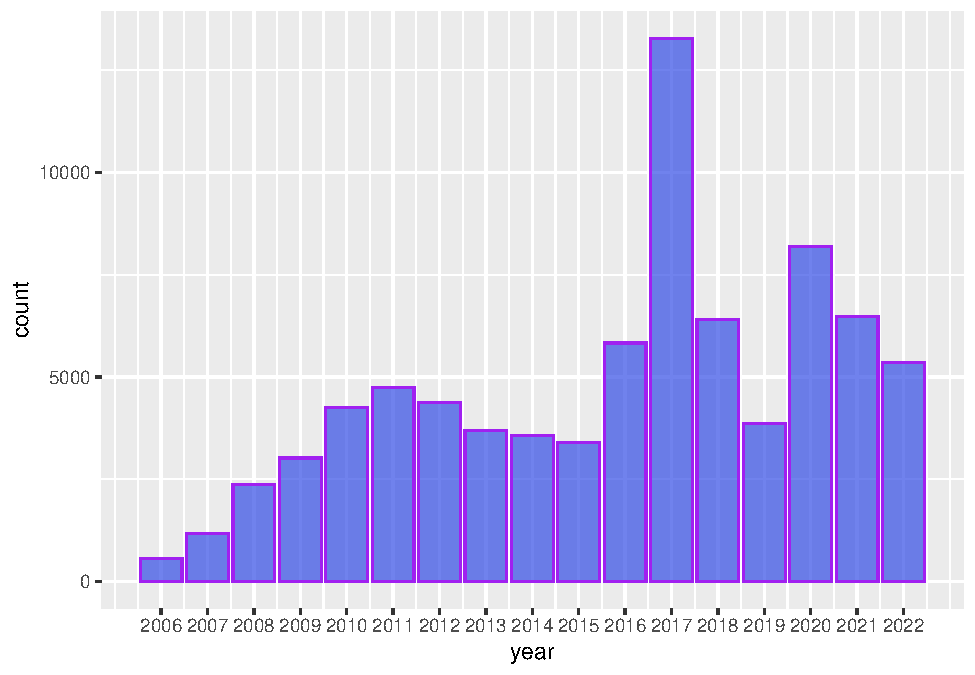
\includegraphics{_main_files/figure-latex/graphs2-1.pdf}

To keep it short, here is a summary table showing if Stakeholders found the RLO(s) they used to be \emph{worth recommending to others}.
We hope there are few NO responses, and many YES responses.

\begin{longtable}[]{@{}llr@{}}
\toprule()
Identity & Recommend & n \\
\midrule()
\endhead
HE student & No & 30 \\
HE student & Yes & 786 \\
Healthcare professional & No & 55 \\
Healthcare professional & Yes & 1311 \\
Other & No & 34 \\
Other & Yes & 767 \\
Patient/Service-user/Carer & No & 2 \\
Patient/Service-user/Carer & Yes & 49 \\
Student & No & 152 \\
Student & Yes & 3164 \\
Tutor/Teacher/Lecturer & No & 5 \\
Tutor/Teacher/Lecturer & Yes & 329 \\
\bottomrule()
\end{longtable}

\begin{longtable}[]{@{}llr@{}}
\toprule()
Identity & RLO & n \\
\midrule()
\endhead
HE student & Helpful & 303 \\
HE student & Not Helpful & 8 \\
HE student & Very Helpful & 474 \\
HE student & Very unhelpful & 10 \\
Healthcare professional & Helpful & 501 \\
Healthcare professional & Not Helpful & 28 \\
Healthcare professional & Very Helpful & 817 \\
Healthcare professional & Very unhelpful & 13 \\
Healthcare professional & Very Unhelpful & 13 \\
Other & Helpful & 322 \\
Other & Not Helpful & 24 \\
Other & Very Helpful & 451 \\
Other & Very unhelpful & 5 \\
Patient/Service-user/Carer & Helpful & 16 \\
Patient/Service-user/Carer & Not Helpful & 1 \\
Patient/Service-user/Carer & Very Helpful & 42 \\
Patient/Service-user/Carer & Very Unhelpful & 2 \\
Student & Helpful & 1392 \\
Student & Not Helpful & 77 \\
Student & Very Helpful & 1863 \\
Student & Very Unhelpful & 9 \\
Tutor/Teacher/Lecturer & Helpful & 97 \\
Tutor/Teacher/Lecturer & Not Helpful & 3 \\
Tutor/Teacher/Lecturer & Very Helpful & 229 \\
Tutor/Teacher/Lecturer & Very unhelpful & 1 \\
\bottomrule()
\end{longtable}

if you don't like boring tables, here is the same data in a graph!

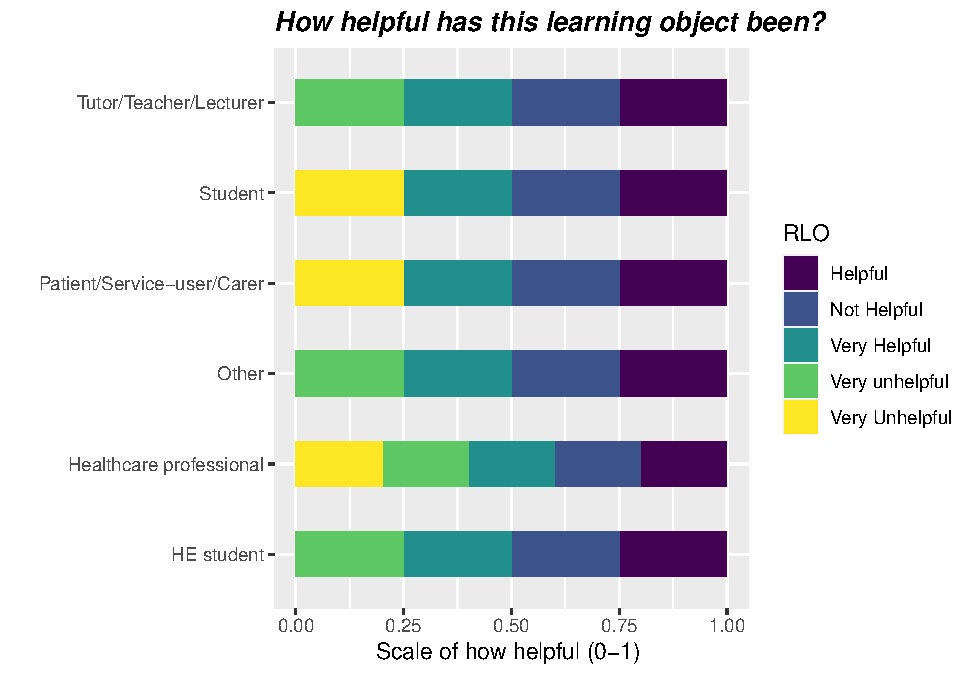
\includegraphics{_main_files/figure-latex/barplot-1.pdf}

\hypertarget{discovering-the-helm-open-rlos}{%
\section{Discovering the HELM Open RLOs}\label{discovering-the-helm-open-rlos}}

\hypertarget{course-learning-recommendations-and-more}{%
\subsection{Course Learning, Recommendations, and more}\label{course-learning-recommendations-and-more}}

The data showed that learners \emph{strongly recommend} the RLO(s) they used to others, but how does this translate?

For the 10\% of data we have, the figure below '\emph{How did you find out about the RLO you used'} shows 700 respondents were recommended from a friend, peer, tutor, or other.

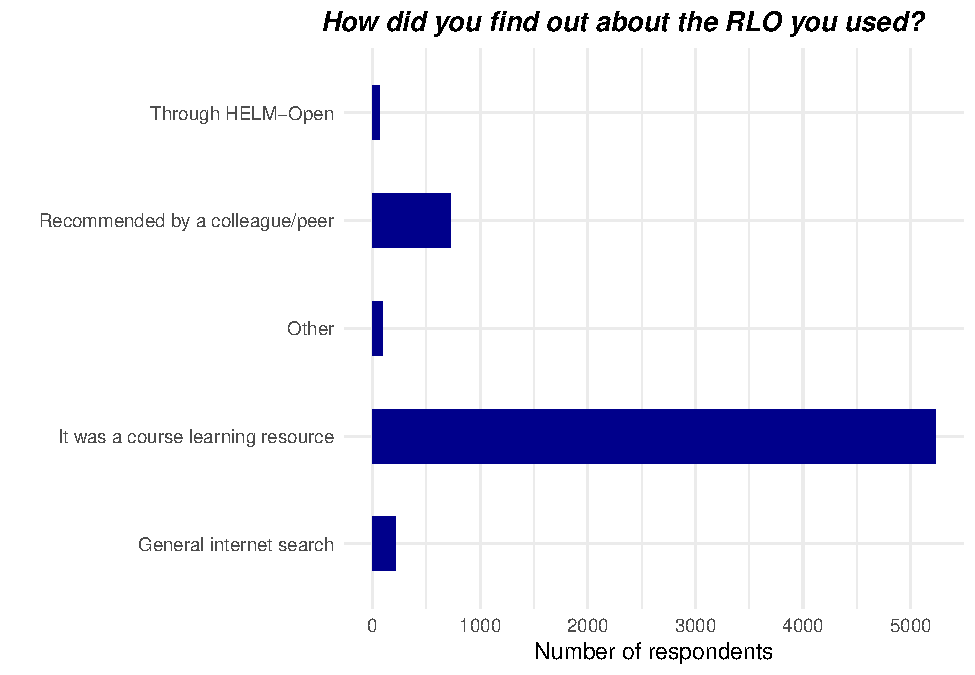
\includegraphics{_main_files/figure-latex/Discovery Section-1.pdf}

This figure also shows how more than 6000 respondents first used the RLOs as instructed by their tutors on their course.

and if you're browsing the internet for information on a healthcare topic and come across \url{https://www.nottingham.ac.uk/helmopen/} :- You're 1 of about 350 people finding about our resources from internet search.
Hopefully that grows, but it seems social networking is the key to sharing these tools.

A random sample of other sources are: Twitter, Aim higher days, Barnardos ignite learning, and, well, `\emph{a random Google photo};'- our online presence seems to be in many places!

UP TO HERE1

\begin{verbatim}
# A tibble: 24 x 3
# Groups:   Identity, dRLO [24]
   Identity                dRLO                                  n
   <chr>                   <chr>                             <int>
 1 HE student              It was a course learning resource    80
 2 HE student              Other                                 2
 3 HE student              Recommended by a colleague/peer       4
 4 HE student              Through HELM-Open                     1
 5 Healthcare professional General internet search               7
 6 Healthcare professional It was a course learning resource   131
 7 Healthcare professional Other                                 3
 8 Healthcare professional Recommended by a colleague/peer      10
 9 Other                   General internet search               8
10 Other                   It was a course learning resource    50
# ... with 14 more rows
\end{verbatim}

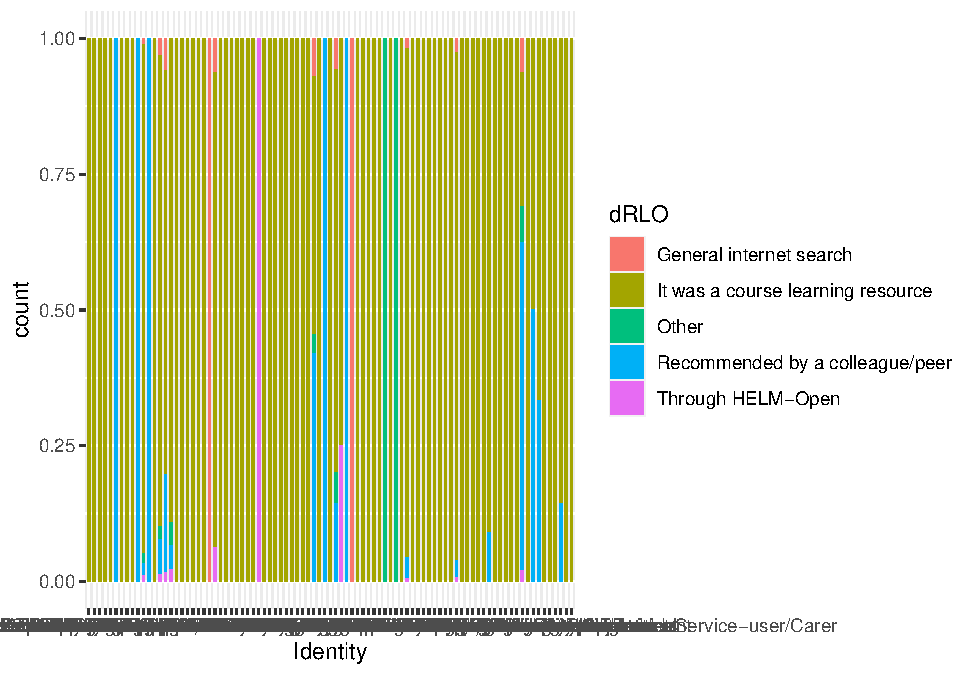
\includegraphics{_main_files/figure-latex/Identity section 1-1.pdf} 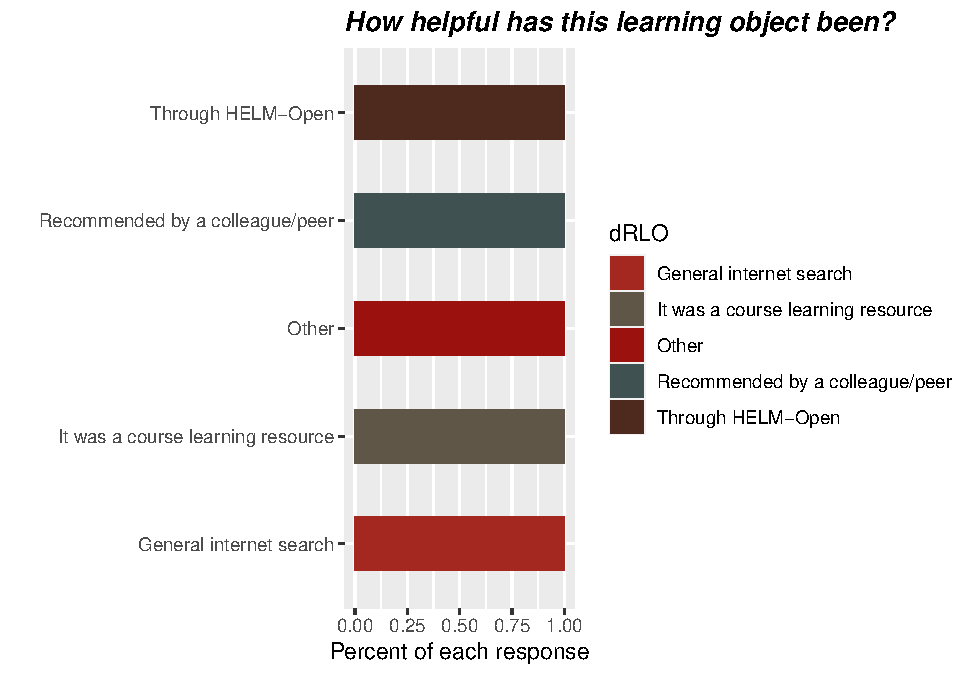
\includegraphics{_main_files/figure-latex/Identity section 1-2.pdf}

\begin{verbatim}
# A tibble: 24 x 3
# Groups:   Identity, dRLO [24]
   Identity                dRLO                                  n
   <chr>                   <chr>                             <int>
 1 HE student              It was a course learning resource    80
 2 HE student              Other                                 2
 3 HE student              Recommended by a colleague/peer       4
 4 HE student              Through HELM-Open                     1
 5 Healthcare professional General internet search               7
 6 Healthcare professional It was a course learning resource   131
 7 Healthcare professional Other                                 3
 8 Healthcare professional Recommended by a colleague/peer      10
 9 Other                   General internet search               8
10 Other                   It was a course learning resource    50
# ... with 14 more rows
\end{verbatim}

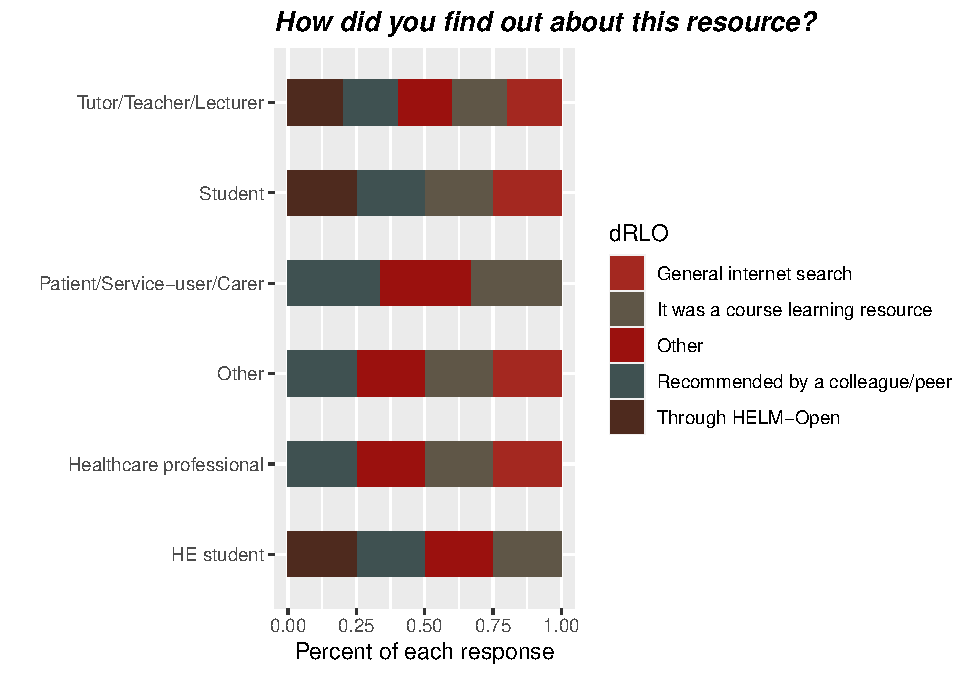
\includegraphics{_main_files/figure-latex/Identity section 1-3.pdf}

\hypertarget{italics-and-bold}{%
\subsection{Italics and bold}\label{italics-and-bold}}

\begin{itemize}
\tightlist
\item
  \emph{Italics} are done like *this* or \_this\_
\item
  \textbf{Bold} is done like **this** or \_\_this\_\_
\item
  \textbf{\emph{Bold and italics}} is done like ***this***, \_\_\_this\_\_\_, or (the most transparent solution, in my opinion) **\_this\_**
\end{itemize}

\hypertarget{inline-code}{%
\subsection{Inline code}\label{inline-code}}

\begin{itemize}
\tightlist
\item
  \texttt{Inline\ code} is created with backticks like \texttt{\textasciigrave{}this\textasciigrave{}}
\end{itemize}

\hypertarget{sub-and-superscript}{%
\subsection{Sub and superscript}\label{sub-and-superscript}}

Sub\textsubscript{2} and super\textsuperscript{2} script is created like this\textasciitilde2\textasciitilde{} and this\^{}2\^{}

\hypertarget{strikethrough}{%
\subsection{Strikethrough}\label{strikethrough}}

\begin{itemize}
\tightlist
\item
  \sout{Strikethrough} is done \textasciitilde\textasciitilde like this\textasciitilde\textasciitilde{}
\end{itemize}

\hypertarget{escaping-aka-what-if-i-need-an-actual-asterisk}{%
\subsection{`Escaping' (aka ``What if I need an actual asterisk?'')}\label{escaping-aka-what-if-i-need-an-actual-asterisk}}

\begin{itemize}
\tightlist
\item
  To include an actual *, \_ or \textbackslash, add another \textbackslash{} in front of them: \textbackslash*, \textbackslash\_, \textbackslash\textbackslash{}
\end{itemize}

\hypertarget{endash-emdash}{%
\subsection{Endash (--), emdash (---)}\label{endash-emdash}}

\begin{itemize}
\tightlist
\item
  -- and --- with -\/- and -\/-\/-
\end{itemize}

\hypertarget{blockquotes}{%
\subsection{Blockquotes}\label{blockquotes}}

Do like this:

\begin{quote}
Put a \textgreater{} in front of the line.
\end{quote}

\hypertarget{headings}{%
\subsection{Headings}\label{headings}}

Section headers are created with \#'s of increasing number, i.e.

\begin{itemize}
\tightlist
\item
  \# First-level heading
\item
  \#\# Second-level heading
\item
  \#\#\# Etc.
\end{itemize}

In PDF output, a level-five heading will turn into a paragraph heading, i.e.~\texttt{\textbackslash{}paragraph\{My\ level-five\ heading\}}, which appears as bold text on the same line as the subsequent paragraph.

\hypertarget{lists}{%
\subsection{Lists}\label{lists}}

Unordered list by starting a line with an * or a -:

\begin{itemize}
\tightlist
\item
  Item 1
\item
  Item 2
\end{itemize}

Ordered lists by starting a line with a number.
Notice that you can mislabel the numbers and \emph{Markdown} will still make the order right in the output:

\begin{enumerate}
\def\labelenumi{\arabic{enumi}.}
\tightlist
\item
  Item 1
\item
  Item 2
\end{enumerate}

To create a sublist, indent the values a bit (at least four spaces or a tab):

\begin{enumerate}
\def\labelenumi{\arabic{enumi}.}
\tightlist
\item
  Item 1
\item
  Item 2
\item
  Item 3

  \begin{itemize}
  \tightlist
  \item
    Item 3a
  \item
    Item 3b
  \end{itemize}
\end{enumerate}

\hypertarget{line-breaks}{%
\subsection{Line breaks}\label{line-breaks}}

The official \emph{Markdown} way to create line breaks is by ending a line with more than two spaces.

Roses are red.
Violets are blue.

This appears on the same line in the output, because we didn't add spaces after red.

Roses are red.\\

Violets are blue.

This appears with a line break because I added spaces after red.

I find this is confusing, so I recommend the alternative way: Ending a line with a backslash will also create a linebreak:

Roses are red.\\

Violets are blue.

To create a new paragraph, you put a blank line.

Therefore, this line starts its own paragraph.

\hypertarget{hyperlinks}{%
\subsection{Hyperlinks}\label{hyperlinks}}

\begin{itemize}
\tightlist
\item
  \href{https://www.google.com}{This is a hyperlink} created by writing the text you want turned into a clickable link in \texttt{{[}square\ brackets\ followed\ by\ a{]}(https://hyperlink-in-parentheses)}
\end{itemize}

\hypertarget{footnotes}{%
\subsection{Footnotes}\label{footnotes}}

\begin{itemize}
\tightlist
\item
  Are created\footnote{my footnote text} by writing either \^{}{[}my footnote text{]} for supplying the footnote content inline, or something like \texttt{{[}\^{}a-random-footnote-label{]}} and supplying the text elsewhere in the format shown below \footnote{This is a random test.}:
\end{itemize}

\texttt{{[}\^{}a-random-footnote-label{]}:\ This\ is\ a\ random\ test.}

\hypertarget{comments}{%
\subsection{Comments}\label{comments}}

To write comments within your text that won't actually be included in the output, use the same syntax as for writing comments in HTML.
That is, .

\hypertarget{math}{%
\subsection{Math}\label{math}}

The syntax for writing math is stolen from LaTeX.
To write a math expression that will be shown \textbf{inline}, enclose it in dollar signs.
- This: \$A = \textbackslash pi*r\^{}\{2\}\$ Becomes: \(A = \pi*r^{2}\)

To write a math expression that will be shown in a block, enclose it in two dollar signs.\\

This: \$\$A = \textbackslash pi*r\^{}\{2\}\$\$

Becomes: \[A = \pi*r^{2}\]

To create numbered equations, put them in an `equation' environment and give them a label with the syntax \texttt{(\textbackslash{}\#eq:label)}, like this:

\begin{Shaded}
\begin{Highlighting}[]
\KeywordTok{\textbackslash{}begin}\NormalTok{\{}\ExtensionTok{equation}\NormalTok{\}}\SpecialStringTok{ }
\SpecialStringTok{  f}\SpecialCharTok{\textbackslash{}left}\SpecialStringTok{(k}\SpecialCharTok{\textbackslash{}right}\SpecialStringTok{) = }\SpecialCharTok{\textbackslash{}binom}\SpecialStringTok{\{n\}\{k\} p\^{}k}\SpecialCharTok{\textbackslash{}left}\SpecialStringTok{(1{-}p}\SpecialCharTok{\textbackslash{}right}\SpecialStringTok{)\^{}\{n{-}k\}}
\SpecialStringTok{  (}\SpecialCharTok{\textbackslash{}\#}\SpecialStringTok{eq:binom)}
\KeywordTok{\textbackslash{}end}\NormalTok{\{}\ExtensionTok{equation}\NormalTok{\} }
\end{Highlighting}
\end{Shaded}

Becomes: \begin{equation}
f\left(k\right)=\binom{n}{k}p^k\left(1-p\right)^{n-k}
\label{eq:binom}
\end{equation}

For more (e.g.~how to theorems), see e.g.~the documentation on \href{https://bookdown.org/yihui/bookdown/markdown-extensions-by-bookdown.html\#equations}{bookdown.org}

\hypertarget{code}{%
\section{Executable code chunks}\label{code}}

The magic of R Markdown is that we can add executable code within our document to make it dynamic.

We do this either as \emph{code chunks} (generally used for loading libraries and data, performing calculations, and adding images, plots, and tables), or \emph{inline code} (generally used for dynamically reporting results within our text).

The syntax of a code chunk is shown in Figure \ref{fig:chunk-parts}.

\begin{figure}[H]
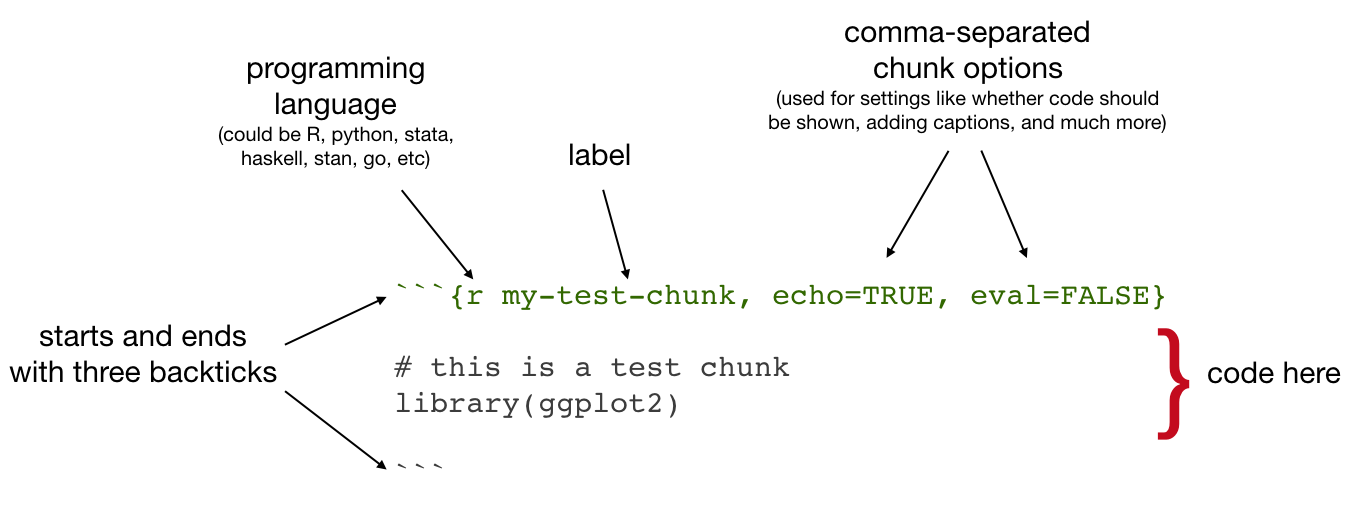
\includegraphics[width=1\linewidth]{figures/sample-content/chunk-parts} \caption{Code chunk syntax}\label{fig:chunk-parts}
\end{figure}

Common chunk options include (see e.g.~\href{https://bookdown.org/yihui/rmarkdown/r-code.html}{bookdown.org}):

\begin{itemize}
\tightlist
\item
  \texttt{echo}: whether or not to display code in knitted output
\item
  \texttt{eval}: whether or to to run the code in the chunk when knitting
\item
  \texttt{include}: whether to include anything from the from a code chunk in the output document
\item
  \texttt{fig.cap}: figure caption
\item
  \texttt{fig.scap}: short figure caption, which will be used in the `List of Figures' in the PDF front matter
\end{itemize}

\textbf{IMPORTANT}: Do \emph{not} use underscoores in your chunk labels - if you do, you are likely to get an error in PDF output saying something like ``! Package caption Error: \textbackslash caption outside float''.

\hypertarget{setup-chunks---setup-images-plots}{%
\subsection{Setup chunks - setup, images, plots}\label{setup-chunks---setup-images-plots}}

An R Markdown document usually begins with a chunk that is used to \textbf{load libraries}, and to \textbf{set default chunk options} with \texttt{knitr::opts\_chunk\$set}.

In your thesis, this will probably happen in \textbf{index.Rmd} and/or as opening chunks in each of your chapters.

\begin{verbatim}
```{r setup, include=FALSE}
# don't show code unless we explicitly set echo = TRUE
knitr::opts_chunk$set(echo = FALSE)

library(tidyverse)
```
\end{verbatim}

\hypertarget{including-images}{%
\subsection{Including images}\label{including-images}}

Code chunks are also used for including images, with \texttt{include\_graphics} from the \texttt{knitr} package, as in Figure \ref{fig:oxford-logo}

\begin{figure}

{\centering 
\includegraphics[width=0.5\linewidth]{figures/sample-content/beltcrest} 

}

\caption{Oxford logo}\label{fig:oxford-logo}
\end{figure}

Useful chunk options for figures include:

\begin{itemize}
\tightlist
\item
  \texttt{out.width} (use with a percentage) for setting the image size
\item
  if you've got an image that gets waaay to big in your output, it will be constrained to the page width by setting \texttt{out.width\ =\ "100\%"}
\end{itemize}

\hypertarget{figure-rotation}{%
\subsubsection*{Figure rotation}\label{figure-rotation}}
\addcontentsline{toc}{subsubsection}{Figure rotation}

You can use the chunk option \texttt{out.extra} to rotate images.

The syntax is different for LaTeX and HTML, so for ease we might start by assigning the right string to a variable that depends on the format you're outputting to:

Then you can reference that variable as the value of \texttt{out.extra} to rotate images, as in Figure \ref{fig:oxford-logo-rotated}.

\begin{figure}

{\centering 
\includegraphics[width=0.5\linewidth,angle=180]{figures/sample-content/beltcrest} 

}

\caption{Oxford logo, rotated}\label{fig:oxford-logo-rotated}
\end{figure}

\hypertarget{including-plots}{%
\subsection{Including plots}\label{including-plots}}

Similarly, code chunks are used for including dynamically generated plots.
You use ordinary code in R or other languages - Figure \ref{fig:cars-plot} shows a plot of the \texttt{cars} dataset of stopping distances for cars at various speeds (this dataset is built in to \textbf{R}).

\begin{figure}
\centering
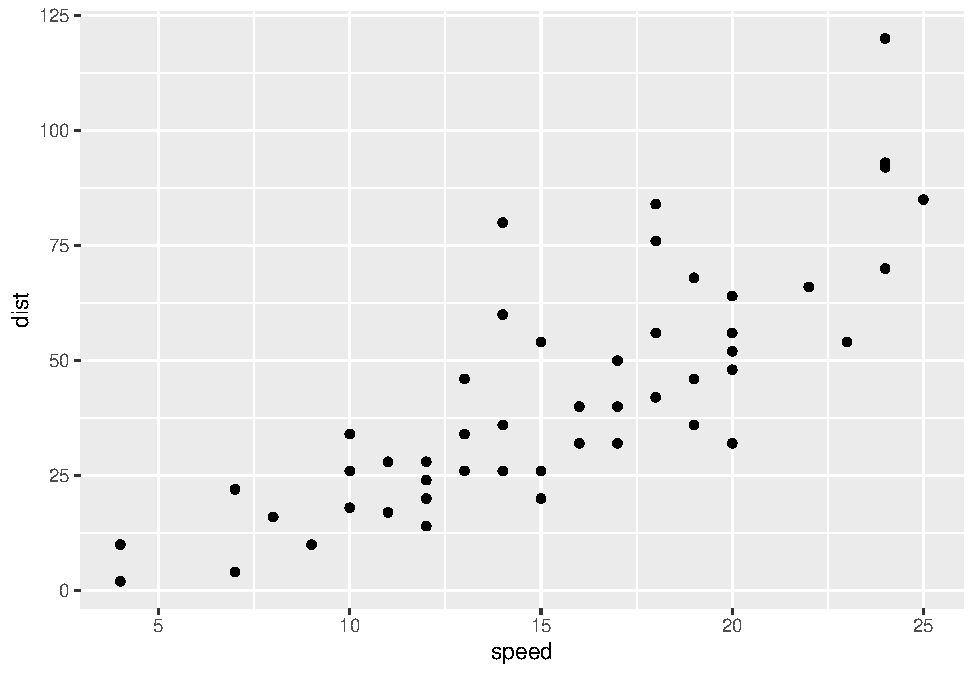
\includegraphics{_main_files/figure-latex/cars-plot-1.pdf}
\caption{\label{fig:cars-plot}A ggplot of car stuff}
\end{figure}

Under the hood, plots are included in your document in the same way as images - when you build the book or knit a chapter, the plot is automatically generated from your code, saved as an image, then included into the output document.

\hypertarget{including-tables}{%
\subsection{Including tables}\label{including-tables}}

Tables are usually included with the \texttt{kable} function from the \texttt{knitr} package.

Table \ref{tab:cars-table} shows the first rows of that cars data - read in your own data, then use this approach to automatically generate tables.

\begin{table}

\caption{\label{tab:cars-table}A knitr kable table}
\centering
\begin{tabular}[t]{r|r}
\hline
speed & dist\\
\hline
4 & 2\\
\hline
4 & 10\\
\hline
7 & 4\\
\hline
7 & 22\\
\hline
8 & 16\\
\hline
9 & 10\\
\hline
\end{tabular}
\end{table}

\begin{itemize}
\tightlist
\item
  Gotcha: when using \href{https://www.rdocumentation.org/packages/knitr/versions/1.21/topics/kable}{\texttt{kable}}, captions are set inside the \texttt{kable} function
\item
  The \texttt{kable} package is often used with the \href{https://cran.r-project.org/web/packages/kableExtra/vignettes/awesome_table_in_html.html}{\texttt{kableExtra}} package
\end{itemize}

\hypertarget{control-positioning}{%
\subsection{Control positioning}\label{control-positioning}}

One thing that may be annoying is the way \emph{R Markdown} handles ``floats'' like tables and figures.
In your PDF output, LaTeX will try to find the best place to put your object based on the text around it and until you're really, truly done writing you should just leave it where it lies.

In general, you should allow LaTeX to do this, but if you really \emph{really} need a figure to be positioned where you put in the document, then you can make LaTeX attempt to do this with the chunk option \texttt{fig.pos="H"}, as in Figure \ref{fig:oxford-logo-controlled}:

\begin{figure}[H]

{\centering 
\includegraphics[width=0.5\linewidth]{figures/sample-content/beltcrest} 

}

\caption{An Oxford logo that LaTeX will try to place at this position in the text}\label{fig:oxford-logo-controlled}
\end{figure}

As anyone who has tried to manually play around with the placement of figures in a Word document knows, this can have lots of side effects with extra spacing on other pages, etc.
Therefore, it is not generally a good idea to do this - only do it when you really need to ensure that an image follows directly under text where you refer to it (in this document, I needed to do this for Figure \ref{fig:latex-font-sizing} in section \ref{max-power}).
For more details, read the relevant section of the \href{https://bookdown.org/yihui/rmarkdown-cookbook/figure-placement.html}{R Markdown Cookbook}.

\hypertarget{executable-inline-code}{%
\section{Executable inline code}\label{executable-inline-code}}

`Inline code' simply means inclusion of code inside text.
The syntax for doing this is \texttt{\textasciigrave{}r\ R\_CODE\textasciigrave{}} For example, \texttt{\textasciigrave{}r\ 4\ +\ 4\textasciigrave{}} will output 8 in your text.

You will usually use this in parts of your thesis where you report results - read in data or results in a code chunk, store things you want to report in a variable, then insert the value of that variable in your text.
For example, we might assign the number of rows in the \texttt{cars} dataset to a variable:

We might then write:\\
``In the \texttt{cars} dataset, we have \texttt{\textasciigrave{}r\ num\_car\_observations\textasciigrave{}} observations.''

Which would output:\\
``In the \texttt{cars} dataset, we have 50 observations.''

\hypertarget{executable-code-in-other-languages-than-r}{%
\section{Executable code in other languages than R}\label{executable-code-in-other-languages-than-r}}

If you want to use other languages than R, such as Python, Julia C++, or SQL, see \href{https://bookdown.org/yihui/rmarkdown-cookbook/other-languages.html}{the relevant section of the \emph{R Markdown Cookbook}}

\hypertarget{cites-and-refs}{%
\chapter{Discussion}\label{cites-and-refs}}

\chaptermark{Citations and cross-refs}

\minitoc 

The usual way to include citations in an \emph{R Markdown} document is to put references in a plain text file with the extension \textbf{.bib}, in \textbf{BibTex} format.\footnote{The bibliography can be in other formats as well, including EndNote (\textbf{.enl}) and RIS (\textbf{.ris}), see \href{https://rmarkdown.rstudio.com/authoring_bibliographies_and_citations.html}{rmarkdown.rstudio.com/authoring\_bibliographies\_and\_citations}.}
Then reference the path to this file in \textbf{index.Rmd}'s YAML header with \texttt{bibliography:\ example.bib}.

Most reference managers can create a .bib file with you references automatically.
However, the \textbf{by far} best reference manager to use with \emph{R Markdown} is \href{https://www.zotero.org}{Zotero} with the \href{https://retorque.re/zotero-better-bibtex/}{Better BibTex plug-in}, because the \texttt{citr} plugin for RStudio (see below) can read references directly from your Zotero library!

Here is an example of an entry in a \textbf{.bib} file:

\begin{Shaded}
\begin{Highlighting}[]
\VariableTok{@article}\NormalTok{\{}\OtherTok{Shea2014}\NormalTok{,}
  \DataTypeTok{author}\NormalTok{ =        \{Shea, Nicholas and Boldt, Annika\},}
  \DataTypeTok{journal}\NormalTok{ =       \{Trends in Cognitive Sciences\},}
  \DataTypeTok{pages}\NormalTok{ =         \{186{-}{-}193\},}
  \DataTypeTok{title}\NormalTok{ =         \{\{Supra{-}personal cognitive control\}\},}
  \DataTypeTok{volume}\NormalTok{ =        \{18\},}
  \DataTypeTok{year}\NormalTok{ =          \{2014\},}
  \DataTypeTok{doi}\NormalTok{ =           \{10.1016/j.tics.2014.01.006\},}
\NormalTok{\}}
\end{Highlighting}
\end{Shaded}

In this entry highlighted section, `Shea2014' is the \textbf{citation identifier}.
To default way to cite an entry in your text is with this syntax: \texttt{{[}@citation-identifier{]}}.

So I might cite some things (\protect\hyperlink{ref-Lottridge2012}{Lottridge et al., 2012}; \protect\hyperlink{ref-Mill1965}{Mill, 1965 {[}1843{]}}; \protect\hyperlink{ref-Shea2014}{Shea et al., 2014}).

\hypertarget{citation-appearance}{%
\subsection{Appearance of citations and references section (pandoc)}\label{citation-appearance}}

By default, \texttt{oxforddown} lets \href{https://pandoc.org}{Pandoc} handle how citations are inserted in your text and the references section.
You can change the appearance of citations and references by specifying a CSL (Citation Style Language) file in the \texttt{csl} metadata field of \textbf{index.Rmd}.
By default, \texttt{oxforddown} by the Americal Psychological Association (7th Edition), which is an author-year format.

With this style, a number of variations on the citation syntax are useful to know:

\begin{itemize}
\tightlist
\item
  Put author names outside the parenthesis

  \begin{itemize}
  \tightlist
  \item
    This: \texttt{@Shea2014\ says\ blah.}
  \item
    Becomes: Shea et al. (\protect\hyperlink{ref-Shea2014}{2014}) says blah.
  \end{itemize}
\item
  Include only the citation-year (in parenthesis)

  \begin{itemize}
  \tightlist
  \item
    This: \texttt{Shea\ et\ al.\ says\ blah\ {[}-@Shea2014{]}}
  \item
    Becomes: Shea et al.~says blah (\protect\hyperlink{ref-Shea2014}{2014})
  \end{itemize}
\item
  Add text and page or chapter references to the citation

  \begin{itemize}
  \tightlist
  \item
    This: \texttt{{[}see\ @Shea2014,\ pp.\ 33-35;\ also\ @Wu2016,\ ch.\ 1{]}}
  \item
    Becomes: Blah blah (see \protect\hyperlink{ref-Shea2014}{Shea et al., 2014, pp. 33--35}; also \protect\hyperlink{ref-Wu2016}{Wu, 2016}, ch.~1).
  \end{itemize}
\end{itemize}

If you want a numerical citation style instead, try \texttt{csl:\ bibliography/transactions-on-computer-human-interaction.csl} or just have a browse through the \href{https://www.zotero.org/styles}{Zotero Style Repository} and look for one you like.
For convenience, you can set the line spacing and the space between the bibliographic entries in the reference section directly from the YAML header in \textbf{index.Rmd}.

If you prefer to use \texttt{biblatex} or \texttt{natbib} to handle references, see \protect\hyperlink{customising-citations}{this chapter}.

\clearpage

\hypertarget{insert-references-easily-with-rstudios-visual-editor}{%
\subsection{Insert references easily with RStudio's Visual Editor}\label{insert-references-easily-with-rstudios-visual-editor}}

For an easy way to insert citations, use RStudio's \href{https://rstudio.github.io/visual-markdown-editing/citations.html}{Visual Editor}.
Make sure you have the latest version of RStudio -- the visual editor was originally really buggy, especially in relation to references, but as per v2022.02.0, it's great!

\hypertarget{cross-referencing}{%
\section{Cross-referencing}\label{cross-referencing}}

We can make cross-references to \textbf{sections} within our document, as well as to \textbf{figures} (images and plots) and \textbf{tables}.

The general cross-referencing syntax is \textbf{\texttt{\textbackslash{}@ref(label)}}

\hypertarget{section-references}{%
\subsection{Section references}\label{section-references}}

Headers are automatically assigned a reference label, which is the text in lower caps separated by dashes. For example, \texttt{\#\ My\ header} is automatically given the label \texttt{my-header}. So \texttt{\#\ My\ header} can be referenced with \texttt{\textbackslash{}@ref(my-section)}

Remember what we wrote in section \ref{citations}?

We can also use \textbf{hyperlink syntax} and add \# before the label, though this is only guaranteed to work properly in HTML output:

\begin{itemize}
\tightlist
\item
  So if we write \texttt{Remember\ what\ we\ wrote\ up\ in\ {[}the\ previous\ section{]}(\#citations)?}
\item
  It becomes Remember what we wrote up in \protect\hyperlink{citations}{the previous section}?
\end{itemize}

\hypertarget{creating-custom-labels}{%
\subsubsection{Creating custom labels}\label{creating-custom-labels}}

It is a very good idea to create \textbf{custom labels} for our sections. This is because the automatically assigned labels will change when we change the titles of the sections - to avoid this, we can create the labels ourselves and leave them untouched if we change the section titles.

We create custom labels by adding \texttt{\{\#label\}} after a header, e.g.~\texttt{\#\ My\ section\ \{\#my-label\}}.
See \protect\hyperlink{cites-and-refs}{our chapter title} for an example. That was section \ref{cites-and-refs}.

\hypertarget{figure-image-and-plot-references}{%
\subsection{Figure (image and plot) references}\label{figure-image-and-plot-references}}

\begin{itemize}
\tightlist
\item
  To refer to figures (i.e.~images and plots) use the syntax \texttt{\textbackslash{}@ref(fig:label)}
\item
  \textbf{GOTCHA}: Figures and tables must have captions if you wish to cross-reference them.
\end{itemize}

Let's add an image:

\begin{figure}

{\centering 
\includegraphics[width=0.65\linewidth]{figures/sample-content/captain} 

}

\caption{A marvel-lous meme}\label{fig:captain}
\end{figure}

We refer to this image with \texttt{\textbackslash{}@ref(fig:captain)}.
So Figure \ref{fig:captain} is \protect\hyperlink{fig:captain}{this image}.

And in Figure \ref{fig:cars-plot} we saw a \protect\hyperlink{fig:cars-plot}{cars plot}.

\hypertarget{table-references}{%
\subsection{Table references}\label{table-references}}

\begin{itemize}
\tightlist
\item
  To refer to tables use the syntax \texttt{\textbackslash{}@ref(tab:label)}
\end{itemize}

Let's include a table:

\begin{table}

\caption{\label{tab:cars-table2}Stopping cars}
\centering
\begin{tabular}[t]{r|r}
\hline
speed & dist\\
\hline
4 & 2\\
\hline
4 & 10\\
\hline
7 & 4\\
\hline
7 & 22\\
\hline
8 & 16\\
\hline
\end{tabular}
\end{table}

We refer to this table with \texttt{\textbackslash{}@ref(tab:cars-table2)}.
So Table \ref{tab:cars-table2} is \protect\hyperlink{tab:cars-table2}{this table}.

And in Table \ref{tab:cars-table} we saw more or less \protect\hyperlink{tab:cars-table}{the same cars table}.

\hypertarget{including-page-numbers}{%
\subsection{Including page numbers}\label{including-page-numbers}}

Finally, in the PDF output we might also want to include the page number of a reference, so that it's easy to find in physical printed output.
LaTeX has a command for this, which looks like this: \texttt{\textbackslash{}pageref\{fig/tab:label\}} (note: curly braces, not parentheses)

When we output to PDF, we can use raw LaTeX directly in our .Rmd files. So if we wanted to include the page of the cars plot we could write:

\begin{itemize}
\tightlist
\item
  This: \texttt{Figure\ \textbackslash{}@ref(fig:cars-plot)\ on\ page\ \textbackslash{}pageref(fig:cars-plot)}
\item
  Becomes: Figure \ref{fig:cars-plot} on page \pageref{fig:cars-plot}
\end{itemize}

\hypertarget{include-page-numbers-only-in-pdf-output}{%
\subsubsection{Include page numbers only in PDF output}\label{include-page-numbers-only-in-pdf-output}}

A problem here is that LaTeX commands don't display in HTML output, so in the gitbook output we'd see simply ``Figure \ref{fig:cars-plot} on page''.

One way to get around this is to use inline R code to insert the text, and use an \texttt{ifelse} statement to check the output format and then insert the appropriate text.

\begin{itemize}
\tightlist
\item
  So this: \texttt{\textasciigrave{}r\ ifelse(knitr::is\_latex\_output(),\ "Figure\ \textbackslash{}\textbackslash{}@ref(fig:cars-plot)\ on\ page\ \textbackslash{}\textbackslash{}pageref\{fig:cars-plot\}",\ "")\textasciigrave{}}
\item
  Inserts this (check this on both PDF and gitbook): Figure \ref{fig:cars-plot} on page \pageref{fig:cars-plot}
\end{itemize}

Note that we need to escape the backslash with another backslash here to get the correct output.

\hypertarget{collaborative-writing}{%
\section{Collaborative writing}\label{collaborative-writing}}

Best practices for collaboration and change tracking when using R Markdown are still an open question.
In the blog post \href{https://livefreeordichotomize.com/2018/09/14/one-year-to-dissertate/}{\textbf{One year to dissertate}} by Lucy D'Agostino, which I highly recommend, the author notes that she knits .Rmd files to a word document, then uses the \texttt{googledrive} R package to send this to Google Drive for comments / revisions from co-authors, then incorporates Google Drive suggestions \emph{by hand} into the .Rmd source files.
This is a bit clunky, and there are ongoing discussions among the \emph{R Markdown} developers about what the best way is to handle collaborative writing (see \href{https://github.com/rstudio/rmarkdown/issues/1463}{issue \#1463} on GitHub, where \href{http://criticmarkup.com}{CriticMarkup} is among the suggestions).

For now, this is an open question in the community of R Markdown users.
I often knit to a format that can easily be imported to Google Docs for comments, then go over suggested revisions and manually incorporate them back in to the .Rmd source files.
For articles, I sometimes upload a near-final draft to \href{https://www.overleaf.com/}{Overleaf}, then collaboratively make final edits to the LaTeX file there.
I suspect some great solution will be developed in the not-to-distant future, probably by the RStudio team.

\hypertarget{additional-resources}{%
\section{Additional resources}\label{additional-resources}}

\begin{itemize}
\item
  \emph{R Markdown: The Definitive Guide} - \url{https://bookdown.org/yihui/rmarkdown/}
\item
  \emph{R for Data Science} - \url{https://r4ds.had.co.nz}
\end{itemize}

\hypertarget{tables}{%
\chapter{Reusable Learning Objects- Exploring Uptake}\label{tables}}

\minitoc 

Here is a (very large) table with all of the currently active RLOS.

\begin{tabular}{llllrllllllllllllllllllllllll}
\toprule
RLO Name & Location & Start Date & SubmissionDate & Year & Identity & Identity\_Other & RLO Helpful & Reason for Using & Discover RLO & Discover\_Other & Problems & Type of Issue & Problem\_Described & Recommend & Advantages & Disadvantages & Rating & Ease of Use & Helpful & Module & Domain & ID Number & Respondent ID & WHICH QUESTIONNAIRE & IP & Latitude & Longitude & City\\
\midrule
01NCTLR Probability and inferential Statistics & NA & 09/12/2010 & 09/12/2010 & 2010 & NA & Ausrtalian teacher looking to use resource & Very Helpful & NA & Through RLO-CETL publicityRecommended by my tutorRecommended by a colleague/peer & NA & NA & NA & NA & Yes & it was clear and helpful & NA & NA & NA & NA & NA & Evidence based practice & NA & 2104178487 & B & 90.244.88.90 & 59.099998 & -3.083330 & Georth\\
01NCTLR Probability and inferential Statistics & NA & 13/04/2013 & 13/04/2013 & 2013 & NA & NA & Helpful & NA & Recommended by my tutor & NA & NA & NA & NA & Yes & It has a video (especially voice; someone speaking) which illustrates and portrays the information very well. & NA & NA & NA & NA & NA & Evidence based practice & NA & 2566726189 & B & 151.226.33.235 & 53.116669 & -3.033330 & Hope\\
01NCTLR Probability and inferential Statistics & NA & 01/05/2014 & 01/05/2014 & 2014 & NA & NA & Helpful & NA & It was a course learning resource & NA & NA & NA & NA & Yes & Exposure to the knowledge that is relevant to my course of study. & NA & NA & NA & NA & NA & Evidence based practice & NA & 3220421679 & B & 31.205.26.150 & 53.250000 & -1.416670 & Chesterfield\\
01NCTLR Probability and inferential Statistics & NA & 04/05/2013 & 04/05/2013 & 2013 & NA & NA & Very Helpful & NA & It was a course learning resource & NA & NA & NA & Calculations involved & Yes & It was practical and tested what I had read. It was also concise and to the point. & NA & NA & NA & NA & NA & Evidence based practice & NA & 2605154704 & B & 86.25.206.148 & 54.973282 & -1.613960 & Newcastle upon Tyne\\
01NCTLR Probability and inferential Statistics & NA & 15/10/2011 & 15/10/2011 & 2011 & NA & NA & Helpful & NA & It was a course learning resource & NA & NA & NA & Flash Shockwave was needed. & Yes & NA & NA & NA & NA & NA & NA & Evidence based practice & NA & 2104178488 & B & 92.20.15.70 & 54.909191 & -1.888450 & Whittonstall\\
\addlinespace
01NCTLR Probability and inferential Statistics & NA & 05/01/2010 & 05/01/2010 & 2010 & NA & NA & Helpful & NA & It was a course learning resource & NA & NA & NA & NA & Yes & I loved  the interactive element and the eclarity of the explanations & NA & NA & NA & NA & NA & Evidence based practice & NA & 2104178426 & B & 78.144.64.158 & 52.184460 & -0.687590 & Warrington\\
\bottomrule
\end{tabular}

\hypertarget{reach-impact-and-qualatative-analysis}{%
\section{Reach, Impact, and Qualatative analysis}\label{reach-impact-and-qualatative-analysis}}

Dealing with tables in LaTeX can be painful.
This section explains the main tricks you need to make the pain go away.

(Note: if you are looking at the eBook version, you will not see much difference in this section, as it is only relevant for PDF output!)

\hypertarget{making-your-table-pretty}{%
\subsection{Making your table pretty}\label{making-your-table-pretty}}

When you use \texttt{kable} to create tables, you will almost certainly want to set the option \texttt{booktabs\ =\ TRUE}.
This makes your table look a million times better:

Compare this to the default style, which looks terrible:

\begin{tabular}{l|r|r|r|r|r|r|r|r|r|r|r}
\hline
  & mpg & cyl & disp & hp & drat & wt & qsec & vs & am & gear & carb\\
\hline
Mazda RX4 & 21.0 & 6 & 160 & 110 & 3.90 & 2.620 & 16.46 & 0 & 1 & 4 & 4\\
\hline
Mazda RX4 Wag & 21.0 & 6 & 160 & 110 & 3.90 & 2.875 & 17.02 & 0 & 1 & 4 & 4\\
\hline
Datsun 710 & 22.8 & 4 & 108 & 93 & 3.85 & 2.320 & 18.61 & 1 & 1 & 4 & 1\\
\hline
Hornet 4 Drive & 21.4 & 6 & 258 & 110 & 3.08 & 3.215 & 19.44 & 1 & 0 & 3 & 1\\
\hline
Hornet Sportabout & 18.7 & 8 & 360 & 175 & 3.15 & 3.440 & 17.02 & 0 & 0 & 3 & 2\\
\hline
Valiant & 18.1 & 6 & 225 & 105 & 2.76 & 3.460 & 20.22 & 1 & 0 & 3 & 1\\
\hline
\end{tabular}

\hypertarget{if-your-table-is-too-wide}{%
\subsection{If your table is too wide}\label{if-your-table-is-too-wide}}

You might find that your table expands into the margins of the page, like the tables above.
Fix this with the \texttt{kable\_styling} function from the \href{https://haozhu233.github.io/kableExtra/}{\texttt{kableExtra}} package:

\begin{table}
\centering
\resizebox{\linewidth}{!}{
\begin{tabular}{lrrrrrrrrrrr}
\toprule
  & mpg & cyl & disp & hp & drat & wt & qsec & vs & am & gear & carb\\
\midrule
Mazda RX4 & 21.0 & 6 & 160 & 110 & 3.90 & 2.620 & 16.46 & 0 & 1 & 4 & 4\\
Mazda RX4 Wag & 21.0 & 6 & 160 & 110 & 3.90 & 2.875 & 17.02 & 0 & 1 & 4 & 4\\
Datsun 710 & 22.8 & 4 & 108 & 93 & 3.85 & 2.320 & 18.61 & 1 & 1 & 4 & 1\\
Hornet 4 Drive & 21.4 & 6 & 258 & 110 & 3.08 & 3.215 & 19.44 & 1 & 0 & 3 & 1\\
Hornet Sportabout & 18.7 & 8 & 360 & 175 & 3.15 & 3.440 & 17.02 & 0 & 0 & 3 & 2\\
\addlinespace
Valiant & 18.1 & 6 & 225 & 105 & 2.76 & 3.460 & 20.22 & 1 & 0 & 3 & 1\\
\bottomrule
\end{tabular}}
\end{table}

This scales down the table to fit the page width.

\hypertarget{if-your-table-is-too-long}{%
\subsection{If your table is too long}\label{if-your-table-is-too-long}}

If your table is too long to fit on a single page, set \texttt{longtable\ =\ TRUE} in the \texttt{kable} function to split the table across multiple pages.

\begin{longtable}{lrrrrrrrr}
\toprule
  & mpg & cyl & disp & hp & drat & wt & qsec & vs\\
\midrule
Mazda RX4 & 21.0 & 6 & 160.0 & 110 & 3.90 & 2.620 & 16.46 & 0\\
Mazda RX4 Wag & 21.0 & 6 & 160.0 & 110 & 3.90 & 2.875 & 17.02 & 0\\
Datsun 710 & 22.8 & 4 & 108.0 & 93 & 3.85 & 2.320 & 18.61 & 1\\
Hornet 4 Drive & 21.4 & 6 & 258.0 & 110 & 3.08 & 3.215 & 19.44 & 1\\
Hornet Sportabout & 18.7 & 8 & 360.0 & 175 & 3.15 & 3.440 & 17.02 & 0\\
\addlinespace
Valiant & 18.1 & 6 & 225.0 & 105 & 2.76 & 3.460 & 20.22 & 1\\
Duster 360 & 14.3 & 8 & 360.0 & 245 & 3.21 & 3.570 & 15.84 & 0\\
Merc 240D & 24.4 & 4 & 146.7 & 62 & 3.69 & 3.190 & 20.00 & 1\\
Merc 230 & 22.8 & 4 & 140.8 & 95 & 3.92 & 3.150 & 22.90 & 1\\
Merc 280 & 19.2 & 6 & 167.6 & 123 & 3.92 & 3.440 & 18.30 & 1\\
\addlinespace
Merc 280C & 17.8 & 6 & 167.6 & 123 & 3.92 & 3.440 & 18.90 & 1\\
Merc 450SE & 16.4 & 8 & 275.8 & 180 & 3.07 & 4.070 & 17.40 & 0\\
Merc 450SL & 17.3 & 8 & 275.8 & 180 & 3.07 & 3.730 & 17.60 & 0\\
Merc 450SLC & 15.2 & 8 & 275.8 & 180 & 3.07 & 3.780 & 18.00 & 0\\
Cadillac Fleetwood & 10.4 & 8 & 472.0 & 205 & 2.93 & 5.250 & 17.98 & 0\\
\addlinespace
Lincoln Continental & 10.4 & 8 & 460.0 & 215 & 3.00 & 5.424 & 17.82 & 0\\
Chrysler Imperial & 14.7 & 8 & 440.0 & 230 & 3.23 & 5.345 & 17.42 & 0\\
Fiat 128 & 32.4 & 4 & 78.7 & 66 & 4.08 & 2.200 & 19.47 & 1\\
Honda Civic & 30.4 & 4 & 75.7 & 52 & 4.93 & 1.615 & 18.52 & 1\\
Toyota Corolla & 33.9 & 4 & 71.1 & 65 & 4.22 & 1.835 & 19.90 & 1\\
\addlinespace
Toyota Corona & 21.5 & 4 & 120.1 & 97 & 3.70 & 2.465 & 20.01 & 1\\
Dodge Challenger & 15.5 & 8 & 318.0 & 150 & 2.76 & 3.520 & 16.87 & 0\\
AMC Javelin & 15.2 & 8 & 304.0 & 150 & 3.15 & 3.435 & 17.30 & 0\\
Camaro Z28 & 13.3 & 8 & 350.0 & 245 & 3.73 & 3.840 & 15.41 & 0\\
Pontiac Firebird & 19.2 & 8 & 400.0 & 175 & 3.08 & 3.845 & 17.05 & 0\\
\addlinespace
Fiat X1-9 & 27.3 & 4 & 79.0 & 66 & 4.08 & 1.935 & 18.90 & 1\\
Porsche 914-2 & 26.0 & 4 & 120.3 & 91 & 4.43 & 2.140 & 16.70 & 0\\
Lotus Europa & 30.4 & 4 & 95.1 & 113 & 3.77 & 1.513 & 16.90 & 1\\
Ford Pantera L & 15.8 & 8 & 351.0 & 264 & 4.22 & 3.170 & 14.50 & 0\\
Ferrari Dino & 19.7 & 6 & 145.0 & 175 & 3.62 & 2.770 & 15.50 & 0\\
\addlinespace
Maserati Bora & 15.0 & 8 & 301.0 & 335 & 3.54 & 3.570 & 14.60 & 0\\
Volvo 142E & 21.4 & 4 & 121.0 & 109 & 4.11 & 2.780 & 18.60 & 1\\
Mazda RX41 & 21.0 & 6 & 160.0 & 110 & 3.90 & 2.620 & 16.46 & 0\\
Mazda RX4 Wag1 & 21.0 & 6 & 160.0 & 110 & 3.90 & 2.875 & 17.02 & 0\\
Datsun 7101 & 22.8 & 4 & 108.0 & 93 & 3.85 & 2.320 & 18.61 & 1\\
\addlinespace
Hornet 4 Drive1 & 21.4 & 6 & 258.0 & 110 & 3.08 & 3.215 & 19.44 & 1\\
Hornet Sportabout1 & 18.7 & 8 & 360.0 & 175 & 3.15 & 3.440 & 17.02 & 0\\
Valiant1 & 18.1 & 6 & 225.0 & 105 & 2.76 & 3.460 & 20.22 & 1\\
Duster 3601 & 14.3 & 8 & 360.0 & 245 & 3.21 & 3.570 & 15.84 & 0\\
Merc 240D1 & 24.4 & 4 & 146.7 & 62 & 3.69 & 3.190 & 20.00 & 1\\
\addlinespace
Merc 2301 & 22.8 & 4 & 140.8 & 95 & 3.92 & 3.150 & 22.90 & 1\\
Merc 2801 & 19.2 & 6 & 167.6 & 123 & 3.92 & 3.440 & 18.30 & 1\\
Merc 280C1 & 17.8 & 6 & 167.6 & 123 & 3.92 & 3.440 & 18.90 & 1\\
Merc 450SE1 & 16.4 & 8 & 275.8 & 180 & 3.07 & 4.070 & 17.40 & 0\\
Merc 450SL1 & 17.3 & 8 & 275.8 & 180 & 3.07 & 3.730 & 17.60 & 0\\
\addlinespace
Merc 450SLC1 & 15.2 & 8 & 275.8 & 180 & 3.07 & 3.780 & 18.00 & 0\\
Cadillac Fleetwood1 & 10.4 & 8 & 472.0 & 205 & 2.93 & 5.250 & 17.98 & 0\\
Lincoln Continental1 & 10.4 & 8 & 460.0 & 215 & 3.00 & 5.424 & 17.82 & 0\\
Chrysler Imperial1 & 14.7 & 8 & 440.0 & 230 & 3.23 & 5.345 & 17.42 & 0\\
Fiat 1281 & 32.4 & 4 & 78.7 & 66 & 4.08 & 2.200 & 19.47 & 1\\
\addlinespace
Honda Civic1 & 30.4 & 4 & 75.7 & 52 & 4.93 & 1.615 & 18.52 & 1\\
Toyota Corolla1 & 33.9 & 4 & 71.1 & 65 & 4.22 & 1.835 & 19.90 & 1\\
Toyota Corona1 & 21.5 & 4 & 120.1 & 97 & 3.70 & 2.465 & 20.01 & 1\\
Dodge Challenger1 & 15.5 & 8 & 318.0 & 150 & 2.76 & 3.520 & 16.87 & 0\\
AMC Javelin1 & 15.2 & 8 & 304.0 & 150 & 3.15 & 3.435 & 17.30 & 0\\
\addlinespace
Camaro Z281 & 13.3 & 8 & 350.0 & 245 & 3.73 & 3.840 & 15.41 & 0\\
Pontiac Firebird1 & 19.2 & 8 & 400.0 & 175 & 3.08 & 3.845 & 17.05 & 0\\
Fiat X1-91 & 27.3 & 4 & 79.0 & 66 & 4.08 & 1.935 & 18.90 & 1\\
Porsche 914-21 & 26.0 & 4 & 120.3 & 91 & 4.43 & 2.140 & 16.70 & 0\\
Lotus Europa1 & 30.4 & 4 & 95.1 & 113 & 3.77 & 1.513 & 16.90 & 1\\
\addlinespace
Ford Pantera L1 & 15.8 & 8 & 351.0 & 264 & 4.22 & 3.170 & 14.50 & 0\\
Ferrari Dino1 & 19.7 & 6 & 145.0 & 175 & 3.62 & 2.770 & 15.50 & 0\\
Maserati Bora1 & 15.0 & 8 & 301.0 & 335 & 3.54 & 3.570 & 14.60 & 0\\
Volvo 142E1 & 21.4 & 4 & 121.0 & 109 & 4.11 & 2.780 & 18.60 & 1\\
\bottomrule
\end{longtable}

When you do this, you'll probably want to make the header repeat on new pages.
Do this with the \texttt{kable\_styling} function from \texttt{kableExtra}:

\begin{longtable}{lrrrrrrrrrrr}
\toprule
  & mpg & cyl & disp & hp & drat & wt & qsec & vs & am & gear & carb\\
\midrule
\endfirsthead
\multicolumn{12}{@{}l}{\textit{(continued)}}\\
\toprule
  & mpg & cyl & disp & hp & drat & wt & qsec & vs & am & gear & carb\\
\midrule
\endhead

\endfoot
\bottomrule
\endlastfoot
Mazda RX4 & 21.0 & 6 & 160.0 & 110 & 3.90 & 2.620 & 16.46 & 0 & 1 & 4 & 4\\
Mazda RX4 Wag & 21.0 & 6 & 160.0 & 110 & 3.90 & 2.875 & 17.02 & 0 & 1 & 4 & 4\\
Datsun 710 & 22.8 & 4 & 108.0 & 93 & 3.85 & 2.320 & 18.61 & 1 & 1 & 4 & 1\\
Hornet 4 Drive & 21.4 & 6 & 258.0 & 110 & 3.08 & 3.215 & 19.44 & 1 & 0 & 3 & 1\\
Hornet Sportabout & 18.7 & 8 & 360.0 & 175 & 3.15 & 3.440 & 17.02 & 0 & 0 & 3 & 2\\
\addlinespace
Valiant & 18.1 & 6 & 225.0 & 105 & 2.76 & 3.460 & 20.22 & 1 & 0 & 3 & 1\\
Duster 360 & 14.3 & 8 & 360.0 & 245 & 3.21 & 3.570 & 15.84 & 0 & 0 & 3 & 4\\
Merc 240D & 24.4 & 4 & 146.7 & 62 & 3.69 & 3.190 & 20.00 & 1 & 0 & 4 & 2\\
Merc 230 & 22.8 & 4 & 140.8 & 95 & 3.92 & 3.150 & 22.90 & 1 & 0 & 4 & 2\\
Merc 280 & 19.2 & 6 & 167.6 & 123 & 3.92 & 3.440 & 18.30 & 1 & 0 & 4 & 4\\
\addlinespace
Merc 280C & 17.8 & 6 & 167.6 & 123 & 3.92 & 3.440 & 18.90 & 1 & 0 & 4 & 4\\
Merc 450SE & 16.4 & 8 & 275.8 & 180 & 3.07 & 4.070 & 17.40 & 0 & 0 & 3 & 3\\
Merc 450SL & 17.3 & 8 & 275.8 & 180 & 3.07 & 3.730 & 17.60 & 0 & 0 & 3 & 3\\
Merc 450SLC & 15.2 & 8 & 275.8 & 180 & 3.07 & 3.780 & 18.00 & 0 & 0 & 3 & 3\\
Cadillac Fleetwood & 10.4 & 8 & 472.0 & 205 & 2.93 & 5.250 & 17.98 & 0 & 0 & 3 & 4\\
\addlinespace
Lincoln Continental & 10.4 & 8 & 460.0 & 215 & 3.00 & 5.424 & 17.82 & 0 & 0 & 3 & 4\\
Chrysler Imperial & 14.7 & 8 & 440.0 & 230 & 3.23 & 5.345 & 17.42 & 0 & 0 & 3 & 4\\
Fiat 128 & 32.4 & 4 & 78.7 & 66 & 4.08 & 2.200 & 19.47 & 1 & 1 & 4 & 1\\
Honda Civic & 30.4 & 4 & 75.7 & 52 & 4.93 & 1.615 & 18.52 & 1 & 1 & 4 & 2\\
Toyota Corolla & 33.9 & 4 & 71.1 & 65 & 4.22 & 1.835 & 19.90 & 1 & 1 & 4 & 1\\
\addlinespace
Toyota Corona & 21.5 & 4 & 120.1 & 97 & 3.70 & 2.465 & 20.01 & 1 & 0 & 3 & 1\\
Dodge Challenger & 15.5 & 8 & 318.0 & 150 & 2.76 & 3.520 & 16.87 & 0 & 0 & 3 & 2\\
AMC Javelin & 15.2 & 8 & 304.0 & 150 & 3.15 & 3.435 & 17.30 & 0 & 0 & 3 & 2\\
Camaro Z28 & 13.3 & 8 & 350.0 & 245 & 3.73 & 3.840 & 15.41 & 0 & 0 & 3 & 4\\
Pontiac Firebird & 19.2 & 8 & 400.0 & 175 & 3.08 & 3.845 & 17.05 & 0 & 0 & 3 & 2\\
\addlinespace
Fiat X1-9 & 27.3 & 4 & 79.0 & 66 & 4.08 & 1.935 & 18.90 & 1 & 1 & 4 & 1\\
Porsche 914-2 & 26.0 & 4 & 120.3 & 91 & 4.43 & 2.140 & 16.70 & 0 & 1 & 5 & 2\\
Lotus Europa & 30.4 & 4 & 95.1 & 113 & 3.77 & 1.513 & 16.90 & 1 & 1 & 5 & 2\\
Ford Pantera L & 15.8 & 8 & 351.0 & 264 & 4.22 & 3.170 & 14.50 & 0 & 1 & 5 & 4\\
Ferrari Dino & 19.7 & 6 & 145.0 & 175 & 3.62 & 2.770 & 15.50 & 0 & 1 & 5 & 6\\
\addlinespace
Maserati Bora & 15.0 & 8 & 301.0 & 335 & 3.54 & 3.570 & 14.60 & 0 & 1 & 5 & 8\\
Volvo 142E & 21.4 & 4 & 121.0 & 109 & 4.11 & 2.780 & 18.60 & 1 & 1 & 4 & 2\\
Mazda RX41 & 21.0 & 6 & 160.0 & 110 & 3.90 & 2.620 & 16.46 & 0 & 1 & 4 & 4\\
Mazda RX4 Wag1 & 21.0 & 6 & 160.0 & 110 & 3.90 & 2.875 & 17.02 & 0 & 1 & 4 & 4\\
Datsun 7101 & 22.8 & 4 & 108.0 & 93 & 3.85 & 2.320 & 18.61 & 1 & 1 & 4 & 1\\
\addlinespace
Hornet 4 Drive1 & 21.4 & 6 & 258.0 & 110 & 3.08 & 3.215 & 19.44 & 1 & 0 & 3 & 1\\
Hornet Sportabout1 & 18.7 & 8 & 360.0 & 175 & 3.15 & 3.440 & 17.02 & 0 & 0 & 3 & 2\\
Valiant1 & 18.1 & 6 & 225.0 & 105 & 2.76 & 3.460 & 20.22 & 1 & 0 & 3 & 1\\
Duster 3601 & 14.3 & 8 & 360.0 & 245 & 3.21 & 3.570 & 15.84 & 0 & 0 & 3 & 4\\
Merc 240D1 & 24.4 & 4 & 146.7 & 62 & 3.69 & 3.190 & 20.00 & 1 & 0 & 4 & 2\\
\addlinespace
Merc 2301 & 22.8 & 4 & 140.8 & 95 & 3.92 & 3.150 & 22.90 & 1 & 0 & 4 & 2\\
Merc 2801 & 19.2 & 6 & 167.6 & 123 & 3.92 & 3.440 & 18.30 & 1 & 0 & 4 & 4\\
Merc 280C1 & 17.8 & 6 & 167.6 & 123 & 3.92 & 3.440 & 18.90 & 1 & 0 & 4 & 4\\
Merc 450SE1 & 16.4 & 8 & 275.8 & 180 & 3.07 & 4.070 & 17.40 & 0 & 0 & 3 & 3\\
Merc 450SL1 & 17.3 & 8 & 275.8 & 180 & 3.07 & 3.730 & 17.60 & 0 & 0 & 3 & 3\\
\addlinespace
Merc 450SLC1 & 15.2 & 8 & 275.8 & 180 & 3.07 & 3.780 & 18.00 & 0 & 0 & 3 & 3\\
Cadillac Fleetwood1 & 10.4 & 8 & 472.0 & 205 & 2.93 & 5.250 & 17.98 & 0 & 0 & 3 & 4\\
Lincoln Continental1 & 10.4 & 8 & 460.0 & 215 & 3.00 & 5.424 & 17.82 & 0 & 0 & 3 & 4\\
Chrysler Imperial1 & 14.7 & 8 & 440.0 & 230 & 3.23 & 5.345 & 17.42 & 0 & 0 & 3 & 4\\
Fiat 1281 & 32.4 & 4 & 78.7 & 66 & 4.08 & 2.200 & 19.47 & 1 & 1 & 4 & 1\\
\addlinespace
Honda Civic1 & 30.4 & 4 & 75.7 & 52 & 4.93 & 1.615 & 18.52 & 1 & 1 & 4 & 2\\
Toyota Corolla1 & 33.9 & 4 & 71.1 & 65 & 4.22 & 1.835 & 19.90 & 1 & 1 & 4 & 1\\
Toyota Corona1 & 21.5 & 4 & 120.1 & 97 & 3.70 & 2.465 & 20.01 & 1 & 0 & 3 & 1\\
Dodge Challenger1 & 15.5 & 8 & 318.0 & 150 & 2.76 & 3.520 & 16.87 & 0 & 0 & 3 & 2\\
AMC Javelin1 & 15.2 & 8 & 304.0 & 150 & 3.15 & 3.435 & 17.30 & 0 & 0 & 3 & 2\\
\addlinespace
Camaro Z281 & 13.3 & 8 & 350.0 & 245 & 3.73 & 3.840 & 15.41 & 0 & 0 & 3 & 4\\
Pontiac Firebird1 & 19.2 & 8 & 400.0 & 175 & 3.08 & 3.845 & 17.05 & 0 & 0 & 3 & 2\\
Fiat X1-91 & 27.3 & 4 & 79.0 & 66 & 4.08 & 1.935 & 18.90 & 1 & 1 & 4 & 1\\
Porsche 914-21 & 26.0 & 4 & 120.3 & 91 & 4.43 & 2.140 & 16.70 & 0 & 1 & 5 & 2\\
Lotus Europa1 & 30.4 & 4 & 95.1 & 113 & 3.77 & 1.513 & 16.90 & 1 & 1 & 5 & 2\\
\addlinespace
Ford Pantera L1 & 15.8 & 8 & 351.0 & 264 & 4.22 & 3.170 & 14.50 & 0 & 1 & 5 & 4\\
Ferrari Dino1 & 19.7 & 6 & 145.0 & 175 & 3.62 & 2.770 & 15.50 & 0 & 1 & 5 & 6\\
Maserati Bora1 & 15.0 & 8 & 301.0 & 335 & 3.54 & 3.570 & 14.60 & 0 & 1 & 5 & 8\\
Volvo 142E1 & 21.4 & 4 & 121.0 & 109 & 4.11 & 2.780 & 18.60 & 1 & 1 & 4 & 2\\*
\end{longtable}

Unfortunately, we cannot use the \texttt{scale\_down} option with a \texttt{longtable}.
So if a \texttt{longtable} is too wide, you can either manually adjust the font size, or show the table in landscape layout.
To adjust the font size, use kableExtra's \texttt{font\_size} option:

\begingroup\fontsize{9}{11}\selectfont

\begin{longtable}{lrrrrrrrrrrr}
\toprule
  & mpg & cyl & disp & hp & drat & wt & qsec & vs & am & gear & carb\\
\midrule
\endfirsthead
\multicolumn{12}{@{}l}{\textit{(continued)}}\\
\toprule
  & mpg & cyl & disp & hp & drat & wt & qsec & vs & am & gear & carb\\
\midrule
\endhead

\endfoot
\bottomrule
\endlastfoot
Mazda RX4 & 21.0 & 6 & 160.0 & 110 & 3.90 & 2.620 & 16.46 & 0 & 1 & 4 & 4\\
Mazda RX4 Wag & 21.0 & 6 & 160.0 & 110 & 3.90 & 2.875 & 17.02 & 0 & 1 & 4 & 4\\
Datsun 710 & 22.8 & 4 & 108.0 & 93 & 3.85 & 2.320 & 18.61 & 1 & 1 & 4 & 1\\
Hornet 4 Drive & 21.4 & 6 & 258.0 & 110 & 3.08 & 3.215 & 19.44 & 1 & 0 & 3 & 1\\
Hornet Sportabout & 18.7 & 8 & 360.0 & 175 & 3.15 & 3.440 & 17.02 & 0 & 0 & 3 & 2\\
\addlinespace
Valiant & 18.1 & 6 & 225.0 & 105 & 2.76 & 3.460 & 20.22 & 1 & 0 & 3 & 1\\
Duster 360 & 14.3 & 8 & 360.0 & 245 & 3.21 & 3.570 & 15.84 & 0 & 0 & 3 & 4\\
Merc 240D & 24.4 & 4 & 146.7 & 62 & 3.69 & 3.190 & 20.00 & 1 & 0 & 4 & 2\\
Merc 230 & 22.8 & 4 & 140.8 & 95 & 3.92 & 3.150 & 22.90 & 1 & 0 & 4 & 2\\
Merc 280 & 19.2 & 6 & 167.6 & 123 & 3.92 & 3.440 & 18.30 & 1 & 0 & 4 & 4\\
\addlinespace
Merc 280C & 17.8 & 6 & 167.6 & 123 & 3.92 & 3.440 & 18.90 & 1 & 0 & 4 & 4\\
Merc 450SE & 16.4 & 8 & 275.8 & 180 & 3.07 & 4.070 & 17.40 & 0 & 0 & 3 & 3\\
Merc 450SL & 17.3 & 8 & 275.8 & 180 & 3.07 & 3.730 & 17.60 & 0 & 0 & 3 & 3\\
Merc 450SLC & 15.2 & 8 & 275.8 & 180 & 3.07 & 3.780 & 18.00 & 0 & 0 & 3 & 3\\
Cadillac Fleetwood & 10.4 & 8 & 472.0 & 205 & 2.93 & 5.250 & 17.98 & 0 & 0 & 3 & 4\\
\addlinespace
Lincoln Continental & 10.4 & 8 & 460.0 & 215 & 3.00 & 5.424 & 17.82 & 0 & 0 & 3 & 4\\
Chrysler Imperial & 14.7 & 8 & 440.0 & 230 & 3.23 & 5.345 & 17.42 & 0 & 0 & 3 & 4\\
Fiat 128 & 32.4 & 4 & 78.7 & 66 & 4.08 & 2.200 & 19.47 & 1 & 1 & 4 & 1\\
Honda Civic & 30.4 & 4 & 75.7 & 52 & 4.93 & 1.615 & 18.52 & 1 & 1 & 4 & 2\\
Toyota Corolla & 33.9 & 4 & 71.1 & 65 & 4.22 & 1.835 & 19.90 & 1 & 1 & 4 & 1\\
\addlinespace
Toyota Corona & 21.5 & 4 & 120.1 & 97 & 3.70 & 2.465 & 20.01 & 1 & 0 & 3 & 1\\
Dodge Challenger & 15.5 & 8 & 318.0 & 150 & 2.76 & 3.520 & 16.87 & 0 & 0 & 3 & 2\\
AMC Javelin & 15.2 & 8 & 304.0 & 150 & 3.15 & 3.435 & 17.30 & 0 & 0 & 3 & 2\\
Camaro Z28 & 13.3 & 8 & 350.0 & 245 & 3.73 & 3.840 & 15.41 & 0 & 0 & 3 & 4\\
Pontiac Firebird & 19.2 & 8 & 400.0 & 175 & 3.08 & 3.845 & 17.05 & 0 & 0 & 3 & 2\\
\addlinespace
Fiat X1-9 & 27.3 & 4 & 79.0 & 66 & 4.08 & 1.935 & 18.90 & 1 & 1 & 4 & 1\\
Porsche 914-2 & 26.0 & 4 & 120.3 & 91 & 4.43 & 2.140 & 16.70 & 0 & 1 & 5 & 2\\
Lotus Europa & 30.4 & 4 & 95.1 & 113 & 3.77 & 1.513 & 16.90 & 1 & 1 & 5 & 2\\
Ford Pantera L & 15.8 & 8 & 351.0 & 264 & 4.22 & 3.170 & 14.50 & 0 & 1 & 5 & 4\\
Ferrari Dino & 19.7 & 6 & 145.0 & 175 & 3.62 & 2.770 & 15.50 & 0 & 1 & 5 & 6\\
\addlinespace
Maserati Bora & 15.0 & 8 & 301.0 & 335 & 3.54 & 3.570 & 14.60 & 0 & 1 & 5 & 8\\
Volvo 142E & 21.4 & 4 & 121.0 & 109 & 4.11 & 2.780 & 18.60 & 1 & 1 & 4 & 2\\
Mazda RX41 & 21.0 & 6 & 160.0 & 110 & 3.90 & 2.620 & 16.46 & 0 & 1 & 4 & 4\\
Mazda RX4 Wag1 & 21.0 & 6 & 160.0 & 110 & 3.90 & 2.875 & 17.02 & 0 & 1 & 4 & 4\\
Datsun 7101 & 22.8 & 4 & 108.0 & 93 & 3.85 & 2.320 & 18.61 & 1 & 1 & 4 & 1\\
\addlinespace
Hornet 4 Drive1 & 21.4 & 6 & 258.0 & 110 & 3.08 & 3.215 & 19.44 & 1 & 0 & 3 & 1\\
Hornet Sportabout1 & 18.7 & 8 & 360.0 & 175 & 3.15 & 3.440 & 17.02 & 0 & 0 & 3 & 2\\
Valiant1 & 18.1 & 6 & 225.0 & 105 & 2.76 & 3.460 & 20.22 & 1 & 0 & 3 & 1\\
Duster 3601 & 14.3 & 8 & 360.0 & 245 & 3.21 & 3.570 & 15.84 & 0 & 0 & 3 & 4\\
Merc 240D1 & 24.4 & 4 & 146.7 & 62 & 3.69 & 3.190 & 20.00 & 1 & 0 & 4 & 2\\
\addlinespace
Merc 2301 & 22.8 & 4 & 140.8 & 95 & 3.92 & 3.150 & 22.90 & 1 & 0 & 4 & 2\\
Merc 2801 & 19.2 & 6 & 167.6 & 123 & 3.92 & 3.440 & 18.30 & 1 & 0 & 4 & 4\\
Merc 280C1 & 17.8 & 6 & 167.6 & 123 & 3.92 & 3.440 & 18.90 & 1 & 0 & 4 & 4\\
Merc 450SE1 & 16.4 & 8 & 275.8 & 180 & 3.07 & 4.070 & 17.40 & 0 & 0 & 3 & 3\\
Merc 450SL1 & 17.3 & 8 & 275.8 & 180 & 3.07 & 3.730 & 17.60 & 0 & 0 & 3 & 3\\
\addlinespace
Merc 450SLC1 & 15.2 & 8 & 275.8 & 180 & 3.07 & 3.780 & 18.00 & 0 & 0 & 3 & 3\\
Cadillac Fleetwood1 & 10.4 & 8 & 472.0 & 205 & 2.93 & 5.250 & 17.98 & 0 & 0 & 3 & 4\\
Lincoln Continental1 & 10.4 & 8 & 460.0 & 215 & 3.00 & 5.424 & 17.82 & 0 & 0 & 3 & 4\\
Chrysler Imperial1 & 14.7 & 8 & 440.0 & 230 & 3.23 & 5.345 & 17.42 & 0 & 0 & 3 & 4\\
Fiat 1281 & 32.4 & 4 & 78.7 & 66 & 4.08 & 2.200 & 19.47 & 1 & 1 & 4 & 1\\
\addlinespace
Honda Civic1 & 30.4 & 4 & 75.7 & 52 & 4.93 & 1.615 & 18.52 & 1 & 1 & 4 & 2\\
Toyota Corolla1 & 33.9 & 4 & 71.1 & 65 & 4.22 & 1.835 & 19.90 & 1 & 1 & 4 & 1\\
Toyota Corona1 & 21.5 & 4 & 120.1 & 97 & 3.70 & 2.465 & 20.01 & 1 & 0 & 3 & 1\\
Dodge Challenger1 & 15.5 & 8 & 318.0 & 150 & 2.76 & 3.520 & 16.87 & 0 & 0 & 3 & 2\\
AMC Javelin1 & 15.2 & 8 & 304.0 & 150 & 3.15 & 3.435 & 17.30 & 0 & 0 & 3 & 2\\
\addlinespace
Camaro Z281 & 13.3 & 8 & 350.0 & 245 & 3.73 & 3.840 & 15.41 & 0 & 0 & 3 & 4\\
Pontiac Firebird1 & 19.2 & 8 & 400.0 & 175 & 3.08 & 3.845 & 17.05 & 0 & 0 & 3 & 2\\
Fiat X1-91 & 27.3 & 4 & 79.0 & 66 & 4.08 & 1.935 & 18.90 & 1 & 1 & 4 & 1\\
Porsche 914-21 & 26.0 & 4 & 120.3 & 91 & 4.43 & 2.140 & 16.70 & 0 & 1 & 5 & 2\\
Lotus Europa1 & 30.4 & 4 & 95.1 & 113 & 3.77 & 1.513 & 16.90 & 1 & 1 & 5 & 2\\
\addlinespace
Ford Pantera L1 & 15.8 & 8 & 351.0 & 264 & 4.22 & 3.170 & 14.50 & 0 & 1 & 5 & 4\\
Ferrari Dino1 & 19.7 & 6 & 145.0 & 175 & 3.62 & 2.770 & 15.50 & 0 & 1 & 5 & 6\\
Maserati Bora1 & 15.0 & 8 & 301.0 & 335 & 3.54 & 3.570 & 14.60 & 0 & 1 & 5 & 8\\
Volvo 142E1 & 21.4 & 4 & 121.0 & 109 & 4.11 & 2.780 & 18.60 & 1 & 1 & 4 & 2\\*
\end{longtable}
\endgroup{}

To put the table in landscape mode, use kableExtra's \texttt{landscape} function:

\begin{landscape}
\begin{longtable}{lrrrrrrrrrrr}
\toprule
  & mpg & cyl & disp & hp & drat & wt & qsec & vs & am & gear & carb\\
\midrule
\endfirsthead
\multicolumn{12}{@{}l}{\textit{(continued)}}\\
\toprule
  & mpg & cyl & disp & hp & drat & wt & qsec & vs & am & gear & carb\\
\midrule
\endhead

\endfoot
\bottomrule
\endlastfoot
Mazda RX4 & 21.0 & 6 & 160.0 & 110 & 3.90 & 2.620 & 16.46 & 0 & 1 & 4 & 4\\
Mazda RX4 Wag & 21.0 & 6 & 160.0 & 110 & 3.90 & 2.875 & 17.02 & 0 & 1 & 4 & 4\\
Datsun 710 & 22.8 & 4 & 108.0 & 93 & 3.85 & 2.320 & 18.61 & 1 & 1 & 4 & 1\\
Hornet 4 Drive & 21.4 & 6 & 258.0 & 110 & 3.08 & 3.215 & 19.44 & 1 & 0 & 3 & 1\\
Hornet Sportabout & 18.7 & 8 & 360.0 & 175 & 3.15 & 3.440 & 17.02 & 0 & 0 & 3 & 2\\
\addlinespace
Valiant & 18.1 & 6 & 225.0 & 105 & 2.76 & 3.460 & 20.22 & 1 & 0 & 3 & 1\\
Duster 360 & 14.3 & 8 & 360.0 & 245 & 3.21 & 3.570 & 15.84 & 0 & 0 & 3 & 4\\
Merc 240D & 24.4 & 4 & 146.7 & 62 & 3.69 & 3.190 & 20.00 & 1 & 0 & 4 & 2\\
Merc 230 & 22.8 & 4 & 140.8 & 95 & 3.92 & 3.150 & 22.90 & 1 & 0 & 4 & 2\\
Merc 280 & 19.2 & 6 & 167.6 & 123 & 3.92 & 3.440 & 18.30 & 1 & 0 & 4 & 4\\
\addlinespace
Merc 280C & 17.8 & 6 & 167.6 & 123 & 3.92 & 3.440 & 18.90 & 1 & 0 & 4 & 4\\
Merc 450SE & 16.4 & 8 & 275.8 & 180 & 3.07 & 4.070 & 17.40 & 0 & 0 & 3 & 3\\
Merc 450SL & 17.3 & 8 & 275.8 & 180 & 3.07 & 3.730 & 17.60 & 0 & 0 & 3 & 3\\
Merc 450SLC & 15.2 & 8 & 275.8 & 180 & 3.07 & 3.780 & 18.00 & 0 & 0 & 3 & 3\\
Cadillac Fleetwood & 10.4 & 8 & 472.0 & 205 & 2.93 & 5.250 & 17.98 & 0 & 0 & 3 & 4\\
\addlinespace
Lincoln Continental & 10.4 & 8 & 460.0 & 215 & 3.00 & 5.424 & 17.82 & 0 & 0 & 3 & 4\\
Chrysler Imperial & 14.7 & 8 & 440.0 & 230 & 3.23 & 5.345 & 17.42 & 0 & 0 & 3 & 4\\
Fiat 128 & 32.4 & 4 & 78.7 & 66 & 4.08 & 2.200 & 19.47 & 1 & 1 & 4 & 1\\
Honda Civic & 30.4 & 4 & 75.7 & 52 & 4.93 & 1.615 & 18.52 & 1 & 1 & 4 & 2\\
Toyota Corolla & 33.9 & 4 & 71.1 & 65 & 4.22 & 1.835 & 19.90 & 1 & 1 & 4 & 1\\
\addlinespace
Toyota Corona & 21.5 & 4 & 120.1 & 97 & 3.70 & 2.465 & 20.01 & 1 & 0 & 3 & 1\\
Dodge Challenger & 15.5 & 8 & 318.0 & 150 & 2.76 & 3.520 & 16.87 & 0 & 0 & 3 & 2\\
AMC Javelin & 15.2 & 8 & 304.0 & 150 & 3.15 & 3.435 & 17.30 & 0 & 0 & 3 & 2\\
Camaro Z28 & 13.3 & 8 & 350.0 & 245 & 3.73 & 3.840 & 15.41 & 0 & 0 & 3 & 4\\
Pontiac Firebird & 19.2 & 8 & 400.0 & 175 & 3.08 & 3.845 & 17.05 & 0 & 0 & 3 & 2\\
\addlinespace
Fiat X1-9 & 27.3 & 4 & 79.0 & 66 & 4.08 & 1.935 & 18.90 & 1 & 1 & 4 & 1\\
Porsche 914-2 & 26.0 & 4 & 120.3 & 91 & 4.43 & 2.140 & 16.70 & 0 & 1 & 5 & 2\\
Lotus Europa & 30.4 & 4 & 95.1 & 113 & 3.77 & 1.513 & 16.90 & 1 & 1 & 5 & 2\\
Ford Pantera L & 15.8 & 8 & 351.0 & 264 & 4.22 & 3.170 & 14.50 & 0 & 1 & 5 & 4\\
Ferrari Dino & 19.7 & 6 & 145.0 & 175 & 3.62 & 2.770 & 15.50 & 0 & 1 & 5 & 6\\
\addlinespace
Maserati Bora & 15.0 & 8 & 301.0 & 335 & 3.54 & 3.570 & 14.60 & 0 & 1 & 5 & 8\\
Volvo 142E & 21.4 & 4 & 121.0 & 109 & 4.11 & 2.780 & 18.60 & 1 & 1 & 4 & 2\\
Mazda RX41 & 21.0 & 6 & 160.0 & 110 & 3.90 & 2.620 & 16.46 & 0 & 1 & 4 & 4\\
Mazda RX4 Wag1 & 21.0 & 6 & 160.0 & 110 & 3.90 & 2.875 & 17.02 & 0 & 1 & 4 & 4\\
Datsun 7101 & 22.8 & 4 & 108.0 & 93 & 3.85 & 2.320 & 18.61 & 1 & 1 & 4 & 1\\
\addlinespace
Hornet 4 Drive1 & 21.4 & 6 & 258.0 & 110 & 3.08 & 3.215 & 19.44 & 1 & 0 & 3 & 1\\
Hornet Sportabout1 & 18.7 & 8 & 360.0 & 175 & 3.15 & 3.440 & 17.02 & 0 & 0 & 3 & 2\\
Valiant1 & 18.1 & 6 & 225.0 & 105 & 2.76 & 3.460 & 20.22 & 1 & 0 & 3 & 1\\
Duster 3601 & 14.3 & 8 & 360.0 & 245 & 3.21 & 3.570 & 15.84 & 0 & 0 & 3 & 4\\
Merc 240D1 & 24.4 & 4 & 146.7 & 62 & 3.69 & 3.190 & 20.00 & 1 & 0 & 4 & 2\\
\addlinespace
Merc 2301 & 22.8 & 4 & 140.8 & 95 & 3.92 & 3.150 & 22.90 & 1 & 0 & 4 & 2\\
Merc 2801 & 19.2 & 6 & 167.6 & 123 & 3.92 & 3.440 & 18.30 & 1 & 0 & 4 & 4\\
Merc 280C1 & 17.8 & 6 & 167.6 & 123 & 3.92 & 3.440 & 18.90 & 1 & 0 & 4 & 4\\
Merc 450SE1 & 16.4 & 8 & 275.8 & 180 & 3.07 & 4.070 & 17.40 & 0 & 0 & 3 & 3\\
Merc 450SL1 & 17.3 & 8 & 275.8 & 180 & 3.07 & 3.730 & 17.60 & 0 & 0 & 3 & 3\\
\addlinespace
Merc 450SLC1 & 15.2 & 8 & 275.8 & 180 & 3.07 & 3.780 & 18.00 & 0 & 0 & 3 & 3\\
Cadillac Fleetwood1 & 10.4 & 8 & 472.0 & 205 & 2.93 & 5.250 & 17.98 & 0 & 0 & 3 & 4\\
Lincoln Continental1 & 10.4 & 8 & 460.0 & 215 & 3.00 & 5.424 & 17.82 & 0 & 0 & 3 & 4\\
Chrysler Imperial1 & 14.7 & 8 & 440.0 & 230 & 3.23 & 5.345 & 17.42 & 0 & 0 & 3 & 4\\
Fiat 1281 & 32.4 & 4 & 78.7 & 66 & 4.08 & 2.200 & 19.47 & 1 & 1 & 4 & 1\\
\addlinespace
Honda Civic1 & 30.4 & 4 & 75.7 & 52 & 4.93 & 1.615 & 18.52 & 1 & 1 & 4 & 2\\
Toyota Corolla1 & 33.9 & 4 & 71.1 & 65 & 4.22 & 1.835 & 19.90 & 1 & 1 & 4 & 1\\
Toyota Corona1 & 21.5 & 4 & 120.1 & 97 & 3.70 & 2.465 & 20.01 & 1 & 0 & 3 & 1\\
Dodge Challenger1 & 15.5 & 8 & 318.0 & 150 & 2.76 & 3.520 & 16.87 & 0 & 0 & 3 & 2\\
AMC Javelin1 & 15.2 & 8 & 304.0 & 150 & 3.15 & 3.435 & 17.30 & 0 & 0 & 3 & 2\\
\addlinespace
Camaro Z281 & 13.3 & 8 & 350.0 & 245 & 3.73 & 3.840 & 15.41 & 0 & 0 & 3 & 4\\
Pontiac Firebird1 & 19.2 & 8 & 400.0 & 175 & 3.08 & 3.845 & 17.05 & 0 & 0 & 3 & 2\\
Fiat X1-91 & 27.3 & 4 & 79.0 & 66 & 4.08 & 1.935 & 18.90 & 1 & 1 & 4 & 1\\
Porsche 914-21 & 26.0 & 4 & 120.3 & 91 & 4.43 & 2.140 & 16.70 & 0 & 1 & 5 & 2\\
Lotus Europa1 & 30.4 & 4 & 95.1 & 113 & 3.77 & 1.513 & 16.90 & 1 & 1 & 5 & 2\\
\addlinespace
Ford Pantera L1 & 15.8 & 8 & 351.0 & 264 & 4.22 & 3.170 & 14.50 & 0 & 1 & 5 & 4\\
Ferrari Dino1 & 19.7 & 6 & 145.0 & 175 & 3.62 & 2.770 & 15.50 & 0 & 1 & 5 & 6\\
Maserati Bora1 & 15.0 & 8 & 301.0 & 335 & 3.54 & 3.570 & 14.60 & 0 & 1 & 5 & 8\\
Volvo 142E1 & 21.4 & 4 & 121.0 & 109 & 4.11 & 2.780 & 18.60 & 1 & 1 & 4 & 2\\*
\end{longtable}
\end{landscape}

\hypertarget{max-power}{%
\subsection{Max power: manually adjust the raw LaTeX output}\label{max-power}}

For total flexibility, you can adjust the raw LaTeX output from \texttt{kable}/\texttt{kableExtra} that generates the table.
Let us consider how we would do this for the example of adjusting the font size if our table is too wide:
Latex has a bunch of standard commands that set an approximate font size, as shown below in Figure \ref{fig:latex-font-sizing}.

\begin{figure}[H]

{\centering 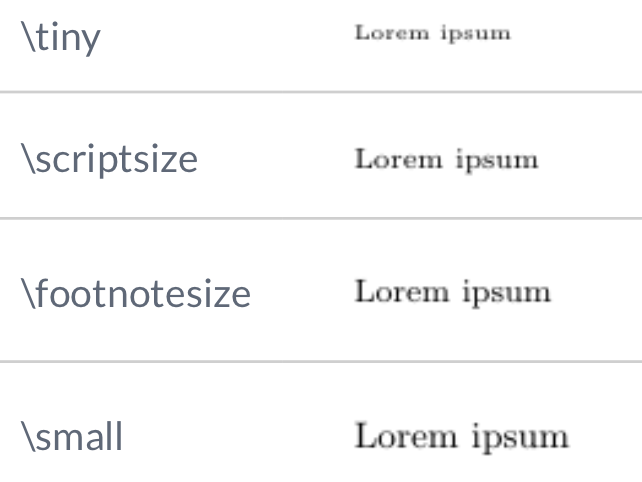
\includegraphics[width=0.5\linewidth]{figures/sample-content/latex_font_sizes} 

}

\caption{Font sizes in LaTeX}\label{fig:latex-font-sizing}
\end{figure}

You could use these to manually adjust the font size in your longtable in two steps:

\begin{enumerate}
\def\labelenumi{\arabic{enumi}.}
\tightlist
\item
  Wrap the longtable environment in, e.g., a \texttt{scriptsize} environment, by doing a string replacement in the output from \texttt{kable}/\texttt{kableExtra}
\item
  Add the attributes that make R Markdown understand that the table is a table (it seems R drops these when we do the string replacement)
\end{enumerate}

\begin{scriptsize}
\begin{longtable}{lrrrrrrrrrrr}
\toprule
  & mpg & cyl & disp & hp & drat & wt & qsec & vs & am & gear & carb\\
\midrule
\endfirsthead
\multicolumn{12}{@{}l}{\textit{(continued)}}\\
\toprule
  & mpg & cyl & disp & hp & drat & wt & qsec & vs & am & gear & carb\\
\midrule
\endhead

\endfoot
\bottomrule
\endlastfoot
Mazda RX4 & 21.0 & 6 & 160.0 & 110 & 3.90 & 2.620 & 16.46 & 0 & 1 & 4 & 4\\
Mazda RX4 Wag & 21.0 & 6 & 160.0 & 110 & 3.90 & 2.875 & 17.02 & 0 & 1 & 4 & 4\\
Datsun 710 & 22.8 & 4 & 108.0 & 93 & 3.85 & 2.320 & 18.61 & 1 & 1 & 4 & 1\\
Hornet 4 Drive & 21.4 & 6 & 258.0 & 110 & 3.08 & 3.215 & 19.44 & 1 & 0 & 3 & 1\\
Hornet Sportabout & 18.7 & 8 & 360.0 & 175 & 3.15 & 3.440 & 17.02 & 0 & 0 & 3 & 2\\
\addlinespace
Valiant & 18.1 & 6 & 225.0 & 105 & 2.76 & 3.460 & 20.22 & 1 & 0 & 3 & 1\\
Duster 360 & 14.3 & 8 & 360.0 & 245 & 3.21 & 3.570 & 15.84 & 0 & 0 & 3 & 4\\
Merc 240D & 24.4 & 4 & 146.7 & 62 & 3.69 & 3.190 & 20.00 & 1 & 0 & 4 & 2\\
Merc 230 & 22.8 & 4 & 140.8 & 95 & 3.92 & 3.150 & 22.90 & 1 & 0 & 4 & 2\\
Merc 280 & 19.2 & 6 & 167.6 & 123 & 3.92 & 3.440 & 18.30 & 1 & 0 & 4 & 4\\
\addlinespace
Merc 280C & 17.8 & 6 & 167.6 & 123 & 3.92 & 3.440 & 18.90 & 1 & 0 & 4 & 4\\
Merc 450SE & 16.4 & 8 & 275.8 & 180 & 3.07 & 4.070 & 17.40 & 0 & 0 & 3 & 3\\
Merc 450SL & 17.3 & 8 & 275.8 & 180 & 3.07 & 3.730 & 17.60 & 0 & 0 & 3 & 3\\
Merc 450SLC & 15.2 & 8 & 275.8 & 180 & 3.07 & 3.780 & 18.00 & 0 & 0 & 3 & 3\\
Cadillac Fleetwood & 10.4 & 8 & 472.0 & 205 & 2.93 & 5.250 & 17.98 & 0 & 0 & 3 & 4\\
\addlinespace
Lincoln Continental & 10.4 & 8 & 460.0 & 215 & 3.00 & 5.424 & 17.82 & 0 & 0 & 3 & 4\\
Chrysler Imperial & 14.7 & 8 & 440.0 & 230 & 3.23 & 5.345 & 17.42 & 0 & 0 & 3 & 4\\
Fiat 128 & 32.4 & 4 & 78.7 & 66 & 4.08 & 2.200 & 19.47 & 1 & 1 & 4 & 1\\
Honda Civic & 30.4 & 4 & 75.7 & 52 & 4.93 & 1.615 & 18.52 & 1 & 1 & 4 & 2\\
Toyota Corolla & 33.9 & 4 & 71.1 & 65 & 4.22 & 1.835 & 19.90 & 1 & 1 & 4 & 1\\
\addlinespace
Toyota Corona & 21.5 & 4 & 120.1 & 97 & 3.70 & 2.465 & 20.01 & 1 & 0 & 3 & 1\\
Dodge Challenger & 15.5 & 8 & 318.0 & 150 & 2.76 & 3.520 & 16.87 & 0 & 0 & 3 & 2\\
AMC Javelin & 15.2 & 8 & 304.0 & 150 & 3.15 & 3.435 & 17.30 & 0 & 0 & 3 & 2\\
Camaro Z28 & 13.3 & 8 & 350.0 & 245 & 3.73 & 3.840 & 15.41 & 0 & 0 & 3 & 4\\
Pontiac Firebird & 19.2 & 8 & 400.0 & 175 & 3.08 & 3.845 & 17.05 & 0 & 0 & 3 & 2\\
\addlinespace
Fiat X1-9 & 27.3 & 4 & 79.0 & 66 & 4.08 & 1.935 & 18.90 & 1 & 1 & 4 & 1\\
Porsche 914-2 & 26.0 & 4 & 120.3 & 91 & 4.43 & 2.140 & 16.70 & 0 & 1 & 5 & 2\\
Lotus Europa & 30.4 & 4 & 95.1 & 113 & 3.77 & 1.513 & 16.90 & 1 & 1 & 5 & 2\\
Ford Pantera L & 15.8 & 8 & 351.0 & 264 & 4.22 & 3.170 & 14.50 & 0 & 1 & 5 & 4\\
Ferrari Dino & 19.7 & 6 & 145.0 & 175 & 3.62 & 2.770 & 15.50 & 0 & 1 & 5 & 6\\
\addlinespace
Maserati Bora & 15.0 & 8 & 301.0 & 335 & 3.54 & 3.570 & 14.60 & 0 & 1 & 5 & 8\\
Volvo 142E & 21.4 & 4 & 121.0 & 109 & 4.11 & 2.780 & 18.60 & 1 & 1 & 4 & 2\\
Mazda RX41 & 21.0 & 6 & 160.0 & 110 & 3.90 & 2.620 & 16.46 & 0 & 1 & 4 & 4\\
Mazda RX4 Wag1 & 21.0 & 6 & 160.0 & 110 & 3.90 & 2.875 & 17.02 & 0 & 1 & 4 & 4\\
Datsun 7101 & 22.8 & 4 & 108.0 & 93 & 3.85 & 2.320 & 18.61 & 1 & 1 & 4 & 1\\
\addlinespace
Hornet 4 Drive1 & 21.4 & 6 & 258.0 & 110 & 3.08 & 3.215 & 19.44 & 1 & 0 & 3 & 1\\
Hornet Sportabout1 & 18.7 & 8 & 360.0 & 175 & 3.15 & 3.440 & 17.02 & 0 & 0 & 3 & 2\\
Valiant1 & 18.1 & 6 & 225.0 & 105 & 2.76 & 3.460 & 20.22 & 1 & 0 & 3 & 1\\
Duster 3601 & 14.3 & 8 & 360.0 & 245 & 3.21 & 3.570 & 15.84 & 0 & 0 & 3 & 4\\
Merc 240D1 & 24.4 & 4 & 146.7 & 62 & 3.69 & 3.190 & 20.00 & 1 & 0 & 4 & 2\\
\addlinespace
Merc 2301 & 22.8 & 4 & 140.8 & 95 & 3.92 & 3.150 & 22.90 & 1 & 0 & 4 & 2\\
Merc 2801 & 19.2 & 6 & 167.6 & 123 & 3.92 & 3.440 & 18.30 & 1 & 0 & 4 & 4\\
Merc 280C1 & 17.8 & 6 & 167.6 & 123 & 3.92 & 3.440 & 18.90 & 1 & 0 & 4 & 4\\
Merc 450SE1 & 16.4 & 8 & 275.8 & 180 & 3.07 & 4.070 & 17.40 & 0 & 0 & 3 & 3\\
Merc 450SL1 & 17.3 & 8 & 275.8 & 180 & 3.07 & 3.730 & 17.60 & 0 & 0 & 3 & 3\\
\addlinespace
Merc 450SLC1 & 15.2 & 8 & 275.8 & 180 & 3.07 & 3.780 & 18.00 & 0 & 0 & 3 & 3\\
Cadillac Fleetwood1 & 10.4 & 8 & 472.0 & 205 & 2.93 & 5.250 & 17.98 & 0 & 0 & 3 & 4\\
Lincoln Continental1 & 10.4 & 8 & 460.0 & 215 & 3.00 & 5.424 & 17.82 & 0 & 0 & 3 & 4\\
Chrysler Imperial1 & 14.7 & 8 & 440.0 & 230 & 3.23 & 5.345 & 17.42 & 0 & 0 & 3 & 4\\
Fiat 1281 & 32.4 & 4 & 78.7 & 66 & 4.08 & 2.200 & 19.47 & 1 & 1 & 4 & 1\\
\addlinespace
Honda Civic1 & 30.4 & 4 & 75.7 & 52 & 4.93 & 1.615 & 18.52 & 1 & 1 & 4 & 2\\
Toyota Corolla1 & 33.9 & 4 & 71.1 & 65 & 4.22 & 1.835 & 19.90 & 1 & 1 & 4 & 1\\
Toyota Corona1 & 21.5 & 4 & 120.1 & 97 & 3.70 & 2.465 & 20.01 & 1 & 0 & 3 & 1\\
Dodge Challenger1 & 15.5 & 8 & 318.0 & 150 & 2.76 & 3.520 & 16.87 & 0 & 0 & 3 & 2\\
AMC Javelin1 & 15.2 & 8 & 304.0 & 150 & 3.15 & 3.435 & 17.30 & 0 & 0 & 3 & 2\\
\addlinespace
Camaro Z281 & 13.3 & 8 & 350.0 & 245 & 3.73 & 3.840 & 15.41 & 0 & 0 & 3 & 4\\
Pontiac Firebird1 & 19.2 & 8 & 400.0 & 175 & 3.08 & 3.845 & 17.05 & 0 & 0 & 3 & 2\\
Fiat X1-91 & 27.3 & 4 & 79.0 & 66 & 4.08 & 1.935 & 18.90 & 1 & 1 & 4 & 1\\
Porsche 914-21 & 26.0 & 4 & 120.3 & 91 & 4.43 & 2.140 & 16.70 & 0 & 1 & 5 & 2\\
Lotus Europa1 & 30.4 & 4 & 95.1 & 113 & 3.77 & 1.513 & 16.90 & 1 & 1 & 5 & 2\\
\addlinespace
Ford Pantera L1 & 15.8 & 8 & 351.0 & 264 & 4.22 & 3.170 & 14.50 & 0 & 1 & 5 & 4\\
Ferrari Dino1 & 19.7 & 6 & 145.0 & 175 & 3.62 & 2.770 & 15.50 & 0 & 1 & 5 & 6\\
Maserati Bora1 & 15.0 & 8 & 301.0 & 335 & 3.54 & 3.570 & 14.60 & 0 & 1 & 5 & 8\\
Volvo 142E1 & 21.4 & 4 & 121.0 & 109 & 4.11 & 2.780 & 18.60 & 1 & 1 & 4 & 2\\*
\end{longtable}
\end{scriptsize}



\hypertarget{text-mining-natural-language-processing-and-sentiment-analysis}{%
\chapter{Text Mining, Natural Language Processing, and Sentiment Analysis}\label{text-mining-natural-language-processing-and-sentiment-analysis}}

\minitoc 

\noindent This chapter describes a number of additional tips and tricks as well as possible customizations to the \texttt{oxforddown} thesis.

\hypertarget{chunk-caching-and-the-_bookdown_files-folder}{%
\section{\texorpdfstring{Chunk caching and the \textbf{\_bookdown\_files} folder}{Chunk caching and the \_bookdown\_files folder}}\label{chunk-caching-and-the-_bookdown_files-folder}}

If you set \texttt{cache=TRUE} in a code chunk, in order to cache its results if it's time-consuming to run see \href{https://bookdown.org/yihui/rmarkdown-cookbook/cache.html}{the R Markdown documentation}, then the files for the caching are stored in the **\_bookdown\_files** folder.

If you don't use caching and you would like to just have the **\_bookdown\_files** folder deleted after the build process is complete, then set \texttt{allow\_cache\ =\ FALSE} in \textbf{index.Rmd}'s call to \texttt{knit\_thesis}.

That is, your YAML should then look like this:

\begin{Shaded}
\begin{Highlighting}[]
\FunctionTok{knit}\KeywordTok{:}\AttributeTok{ (function(input, ...) \{}
\AttributeTok{    thesis\_formats \textless{}{-} "pdf";}
\AttributeTok{    }
\AttributeTok{    source("scripts\_and\_filters/knit{-}functions.R");}
\AttributeTok{    knit\_thesis(input, thesis\_formats, allow\_cache = FALSE, ...)}
\AttributeTok{  \})}
\end{Highlighting}
\end{Shaded}

\hypertarget{front-matter}{%
\section{Front matter}\label{front-matter}}

\hypertarget{shorten-captions-shown-in-the-list-of-figures-pdf}{%
\subsection{Shorten captions shown in the list of figures (PDF)}\label{shorten-captions-shown-in-the-list-of-figures-pdf}}

You might want your list of figures (which follows the table of contents) to have shorter (or just different) figure descriptions than the actual figure captions.

Do this using the chunk option \texttt{fig.scap} (`short caption'), for example \texttt{\{r\ captain-image,\ fig.cap="A\ very\ long\ and\ descriptive\ (and\ potentially\ boring)\ caption\ that\ doesn\textquotesingle{}t\ fit\ in\ the\ list\ of\ figures,\ but\ helps\ the\ reader\ understand\ what\ the\ figure\ communicates.",\ fig.scap="A\ concise\ description\ for\ the\ list\ of\ figures"}

\hypertarget{shorten-captions-shown-in-the-list-of-tables-pdf}{%
\subsection{Shorten captions shown in the list of tables (PDF)}\label{shorten-captions-shown-in-the-list-of-tables-pdf}}

You might want your list of tables (which follows the list of figures in your thesis front matter) to have shorter (or just different) table descriptions than the actual table captions.

If you are using \texttt{knitr::kable} to generate a table, you can do this with the argument \texttt{caption.short}, e.g.:

\begin{Shaded}
\begin{Highlighting}[]
\NormalTok{knitr}\SpecialCharTok{::}\FunctionTok{kable}\NormalTok{(mtcars,}
              \AttributeTok{caption =} \StringTok{"A very long and descriptive (and potentially}
\StringTok{              boring) caption that doesn\textquotesingle{}t fit in the list of figures,}
\StringTok{              but helps the reader understand what the figure }
\StringTok{              communicates."}\NormalTok{,}
              \AttributeTok{caption.short =} \StringTok{"A concise description for the list of tables"}\NormalTok{)}
\end{Highlighting}
\end{Shaded}

\hypertarget{shorten-running-header-pdf}{%
\section{Shorten running header (PDF)}\label{shorten-running-header-pdf}}

You might want a chapter's running header (i.e.~the header showing the title of the current chapter at the top of page) to be shorter (or just different) to the actual chapter title.

Do this by adding the latex command \texttt{\textbackslash{}chaptermark\{My\ shorter\ version\}} after your chapter title.

For example, chapter \ref{cites-and-refs}`s running header is simply 'Cites and cross-refs', because it begins like this:

\begin{Shaded}
\begin{Highlighting}[]
\FunctionTok{\# Citations, cross{-}references, and collaboration \{\#cites{-}and{-}refs\} }
\NormalTok{\textbackslash{}chaptermark\{Cites and cross{-}refs\}}
\end{Highlighting}
\end{Shaded}

\hypertarget{unnumbered-chapters}{%
\section{Unnumbered chapters}\label{unnumbered-chapters}}

To make chapters unnumbered (normally only relevant to the Introduction and/or the Conclusion), follow the chapter header with \texttt{\{-\}}, e.g.~\texttt{\#\ Introduction\ \{-\}}.

When you do this, you must also follow the heading with these two latex commands:

\begin{Shaded}
\begin{Highlighting}[]
\FunctionTok{\textbackslash{}adjustmtc}
\FunctionTok{\textbackslash{}markboth}\NormalTok{\{The Name of Your Unnumbered Chapter\}\{\}}
\end{Highlighting}
\end{Shaded}

Otherwise the chapter's mini table of contents and the running header will show the previous chapter.

\hypertarget{beginning-chapters-with-quotes-pdf}{%
\section{Beginning chapters with quotes (PDF)}\label{beginning-chapters-with-quotes-pdf}}

The OxThesis LaTeX template lets you inject some wittiness into your thesis by including a block of type \texttt{savequote} at the beginning of chapters.
To do this, use the syntax \texttt{\textasciigrave{}\textasciigrave{}\textasciigrave{}\{block\ type=\textquotesingle{}savequote\textquotesingle{}\}}.\footnote{For more on custom block types, see the relevant section in \href{https://bookdown.org/yihui/bookdown/custom-blocks.html}{\emph{Authoring Books with R Markdown}}.}

Add the reference for the quote with the chunk option \texttt{quote\_author="my\ author\ name"}.
You will also want to add the chunk option \texttt{include=knitr::is\_latex\_output()} so that quotes are only included in PDF output.

It's not possible to use markdown syntax inside chunk options, so if you want to e.g.~italicise a book name in the reference use a \href{https://bookdown.org/yihui/bookdown/markdown-extensions-by-bookdown.html\#text-references}{`text reference'}: Create a named piece of text with `(ref:label-name) My text', then point to this in the chunk option with \texttt{quote\_author=\textquotesingle{}(ref:label-name)\textquotesingle{}}.

\hypertarget{highlighting-corrections-html-pdf}{%
\section{Highlighting corrections (HTML \& PDF)}\label{highlighting-corrections-html-pdf}}

For when it comes time to do corrections, you may want to highlight changes made when you submit a post-viva, corrected copy to your examiners so they can quickly verify you've completed the task.
You can do so like this:

\hypertarget{short-inline-corrections}{%
\subsection{Short, inline corrections}\label{short-inline-corrections}}

Highlight \textbf{short, inline corrections} by doing \texttt{{[}like\ this{]}\{.correction\}} --- the text between the square brackets will then \hl{be highlighted in blue} in the output.

Note that pandoc might get confused by citations and cross-references inside inline corrections.
In particular, it might get confused by \texttt{"{[}what\ @Shea2014\ said{]}\{.correction\}"} which becomes \hl{what Shea et al. (\protect\hyperlink{ref-Shea2014}{2014}) said}
In such cases, you can use LaTeX syntax directly.
The correction highlighting uses the \href{https://ctan.org/pkg/soul}{soul} package, so you can do like this:

\begin{itemize}
\tightlist
\item
  If using biblatex for references, use \texttt{"\textbackslash{}hl\{what\ \textbackslash{}textcite\{Shea2014\}\ said\}}
\item
  If using natbib for references, use \texttt{"\textbackslash{}hl\{what\ \textbackslash{}cite\{Shea2014\}\ said\}}
\end{itemize}

Using raw LaTeX has the drawback of corrections then not showing up in HTML output at all, but you might only care about correction highlighting in the PDF for your examiners anyway!

\hypertarget{blocks-of-added-or-changed-material}{%
\subsection{Blocks of added or changed material}\label{blocks-of-added-or-changed-material}}

Highlight entire \textbf{blocks of added or changed material} by putting them in a block of type \texttt{correction}, using the syntax \texttt{\textasciigrave{}\textasciigrave{}\textasciigrave{}\{block\ type=\textquotesingle{}correction\textquotesingle{}\}}.\footnote{In the \textbf{.tex} file for PDF output, this will put the content between \texttt{\textbackslash{}begin\{correction\}} and \texttt{\textbackslash{}end\{correction\}}; in gitbook output it will be put between \texttt{\textless{}div\ class="correction"\textgreater{}} and \texttt{\textless{}/div\textgreater{}}.}
Like so:

\emph{Note that correction blocks cannot be included in word output.}

\hypertarget{stopping-corrections-from-being-highlighted}{%
\subsection{Stopping corrections from being highlighted}\label{stopping-corrections-from-being-highlighted}}

To turn off correction highlighting, go to the YAML header of \textbf{index.Rmd}, then:

\begin{itemize}
\tightlist
\item
  PDF output: set \texttt{corrections:\ false}\\
\item
  HTML output: remove or comment out \texttt{-\ templates/corrections.css}
\end{itemize}

\hypertarget{apply-custom-font-color-and-highlighting-to-text-html-pdf}{%
\section{Apply custom font color and highlighting to text (HTML \& PDF)}\label{apply-custom-font-color-and-highlighting-to-text-html-pdf}}

The lua filter that adds the functionality to highlight corrections adds two more tricks:
you can apply your own choice of colour to highlight text, or change the font color.
The syntax is as follows:

\begin{quote}
Here's \texttt{{[}some\ text\ in\ pink\ highlighting{]}\{highlight="pink"\}}\\
Becomes: Here's \sethlcolor{pink}\hl{some text in pink highlighting}\sethlcolor{correctioncolor}.
\end{quote}

\begin{quote}
\texttt{{[}Here\textquotesingle{}s\ some\ text\ with\ blue\ font{]}\{color="blue"\}}\strut \\
Becomes: \textcolor{blue}{Here's some text with blue font}
\end{quote}

\begin{quote}
Finally --- never, ever actually do this -- \texttt{{[}here\textquotesingle{}s\ some\ text\ with\ black\ highlighting\ and\ yellow\ font{]}\{highlight="black"\ color="yellow"\}}\\
Becomes: \textcolor{yellow}{\sethlcolor{black}\hl{here's some text with black highlighting and yellow font}\sethlcolor{correctioncolor}}
\end{quote}

The file \textbf{scripts\_and\_filters/colour\_and\_highlight.lua} implements this, if you want to fiddle around with it.
It works with both PDF and HTML output.

\hypertarget{adding-a-second-abstract-pdf}{%
\section{Adding a second abstract (PDF)}\label{adding-a-second-abstract-pdf}}

You may need two abstracts in your thesis, if you e.g.~need both an abstract in English and some other language.

You can add a second abstract in \textbf{index.Rmd} like so:

\begin{Shaded}
\begin{Highlighting}[]
\FunctionTok{abstract{-}second{-}heading}\KeywordTok{:}\AttributeTok{ }\StringTok{"Resumé"}
\FunctionTok{abstract{-}second}\KeywordTok{:}\AttributeTok{ }\StringTok{"This is the second abstract, for example in beautiful French."}\AttributeTok{ }
\end{Highlighting}
\end{Shaded}

\hypertarget{embed-pdf}{%
\section{Including another paper in your thesis - embed a PDF document}\label{embed-pdf}}

You may want to embed existing PDF documents into the thesis, for example if your department allows a `portfolio' style thesis and you need to include an existing typeset publication as a chapter.

In gitbook output, you can simply use \texttt{knitr::include\_graphics} and it should include a scrollable (and downloadable) PDF.
You will probably want to set the chunk options \texttt{out.width=\textquotesingle{}100\%\textquotesingle{}} and \texttt{out.height=\textquotesingle{}1000px\textquotesingle{}}:

In LaTeX output, however, this approach can cause odd behaviour.
Therefore, when you build your thesis to PDF, split the PDF into an alphanumerically sorted sequence of \textbf{single-page} PDF files (you can do this automatically with the package \texttt{pdftools}). You can then use the appropriate LaTeX command to insert them, as shown below (for brevity, in the \texttt{oxforddown} PDF sample content we're only including two pages).
\emph{Note that the chunk option \texttt{results=\textquotesingle{}asis\textquotesingle{}} must be set.}
You may also want to remove margins from the PDF files, which you can do with Adobe Acrobat (paid version) and likely other software.

\begin{Shaded}
\begin{Highlighting}[]
\CommentTok{\# install.packages(pdftools)}
\CommentTok{\# split PDF into pages stored in figures/sample{-}content/pdf\_embed\_example/split/}
\CommentTok{\# pdftools::pdf\_split("figures/sample{-}content/pdf\_embed\_example/Lyngs2020\_FB.pdf",}
\CommentTok{\#        output = "figures/sample{-}content/pdf\_embed\_example/split/")}

\CommentTok{\# grab the pages}
\NormalTok{pages }\OtherTok{\textless{}{-}} \FunctionTok{list.files}\NormalTok{(}\StringTok{"figures/sample{-}content/pdf\_embed\_example/split"}\NormalTok{, }\AttributeTok{full.names =} \ConstantTok{TRUE}\NormalTok{)}

\CommentTok{\# set how wide you want the inserted PDFs to be: }
\CommentTok{\# 1.0 is 100 per cent of the oxforddown PDF page width;}
\CommentTok{\# you may want to make it a bit bigger}
\NormalTok{pdf\_width }\OtherTok{\textless{}{-}} \FloatTok{1.2}

\CommentTok{\# for each PDF page, insert it nicely and}
\CommentTok{\# end with a page break}
\FunctionTok{cat}\NormalTok{(stringr}\SpecialCharTok{::}\FunctionTok{str\_c}\NormalTok{(}\StringTok{"}\SpecialCharTok{\textbackslash{}\textbackslash{}}\StringTok{newpage }\SpecialCharTok{\textbackslash{}\textbackslash{}}\StringTok{begin\{center\} }\SpecialCharTok{\textbackslash{}\textbackslash{}}\StringTok{makebox[}\SpecialCharTok{\textbackslash{}\textbackslash{}}\StringTok{linewidth][c]\{}\SpecialCharTok{\textbackslash{}\textbackslash{}}\StringTok{includegraphics[width="}\NormalTok{, pdf\_width, }\StringTok{"}\SpecialCharTok{\textbackslash{}\textbackslash{}}\StringTok{linewidth]\{"}\NormalTok{, pages, }\StringTok{"\}\} }\SpecialCharTok{\textbackslash{}\textbackslash{}}\StringTok{end\{center\}"}\NormalTok{))}
\end{Highlighting}
\end{Shaded}

\newpage \begin{center} \makebox[\linewidth][c]{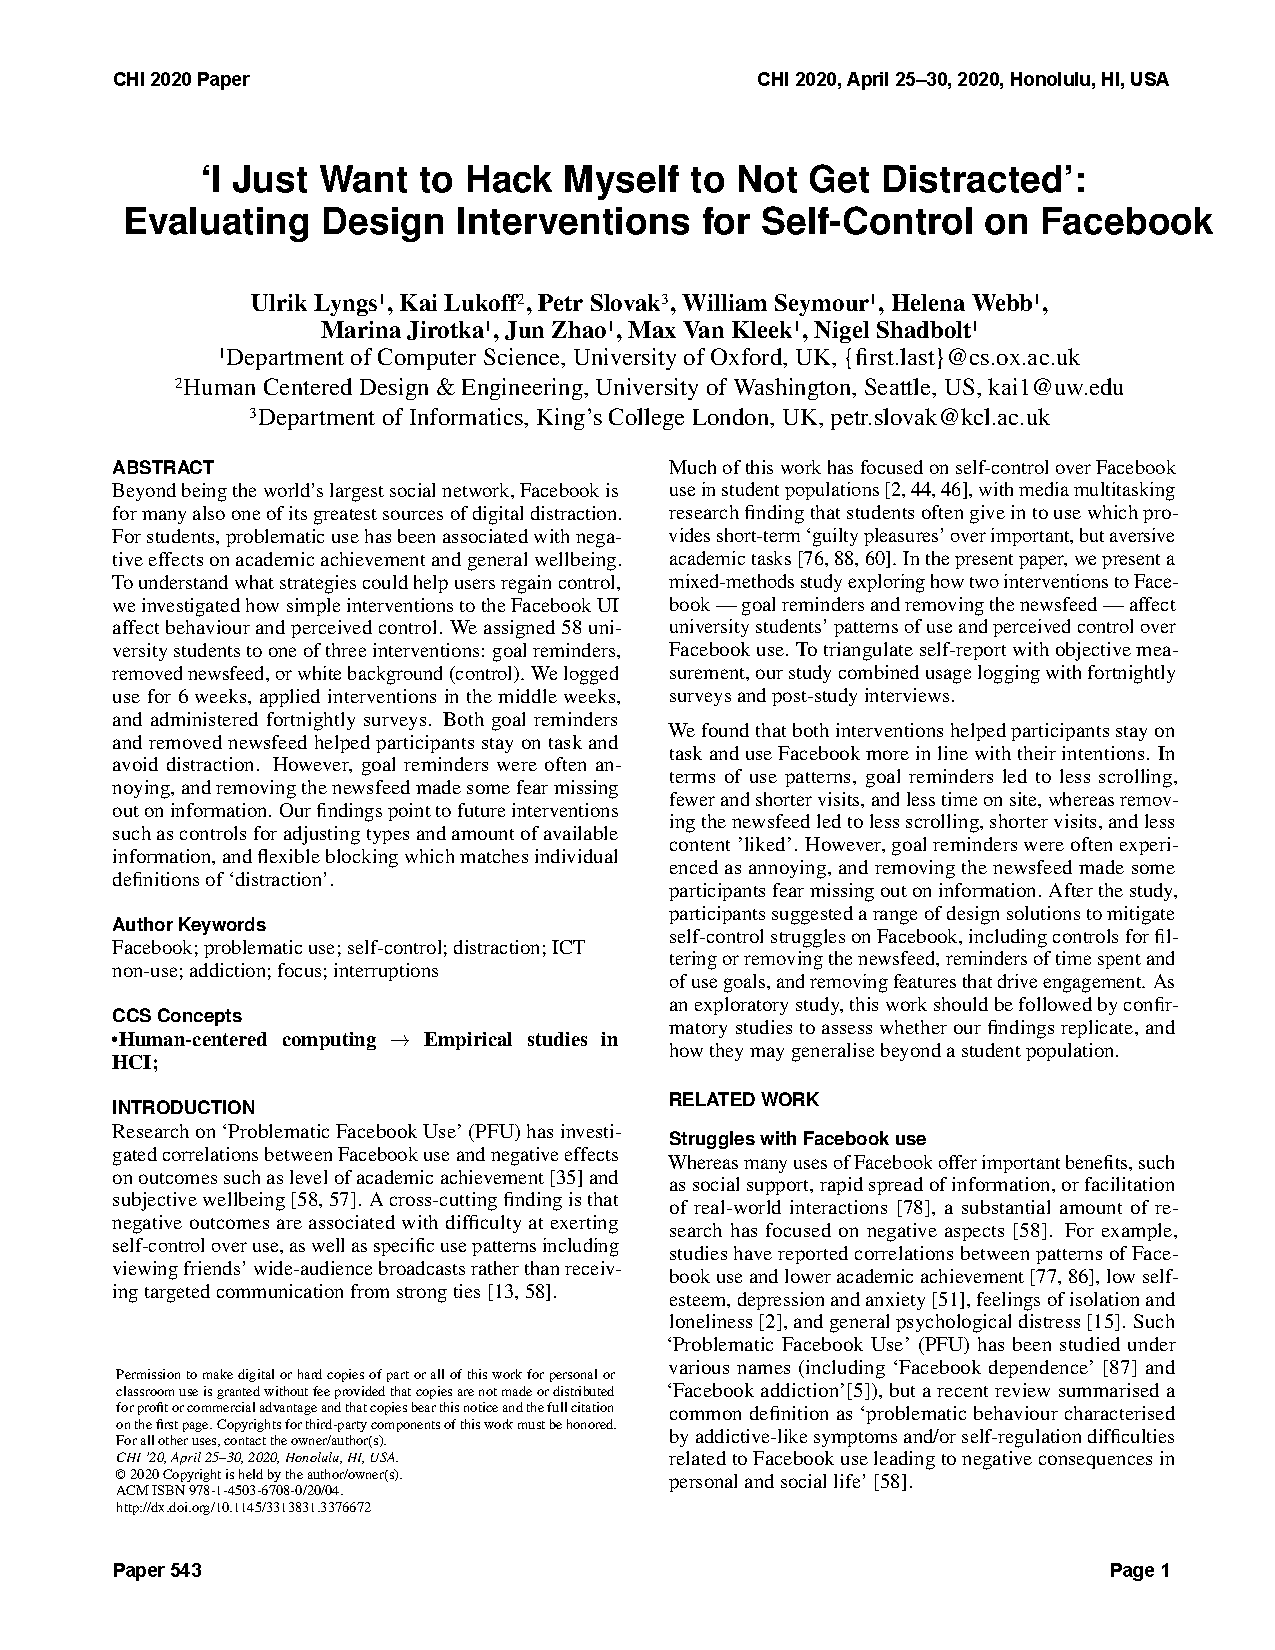
\includegraphics[width=1.2\linewidth]{figures/sample-content/pdf_embed_example/split/_000000000000001.pdf}} \end{center} \newpage \begin{center} \makebox[\linewidth][c]{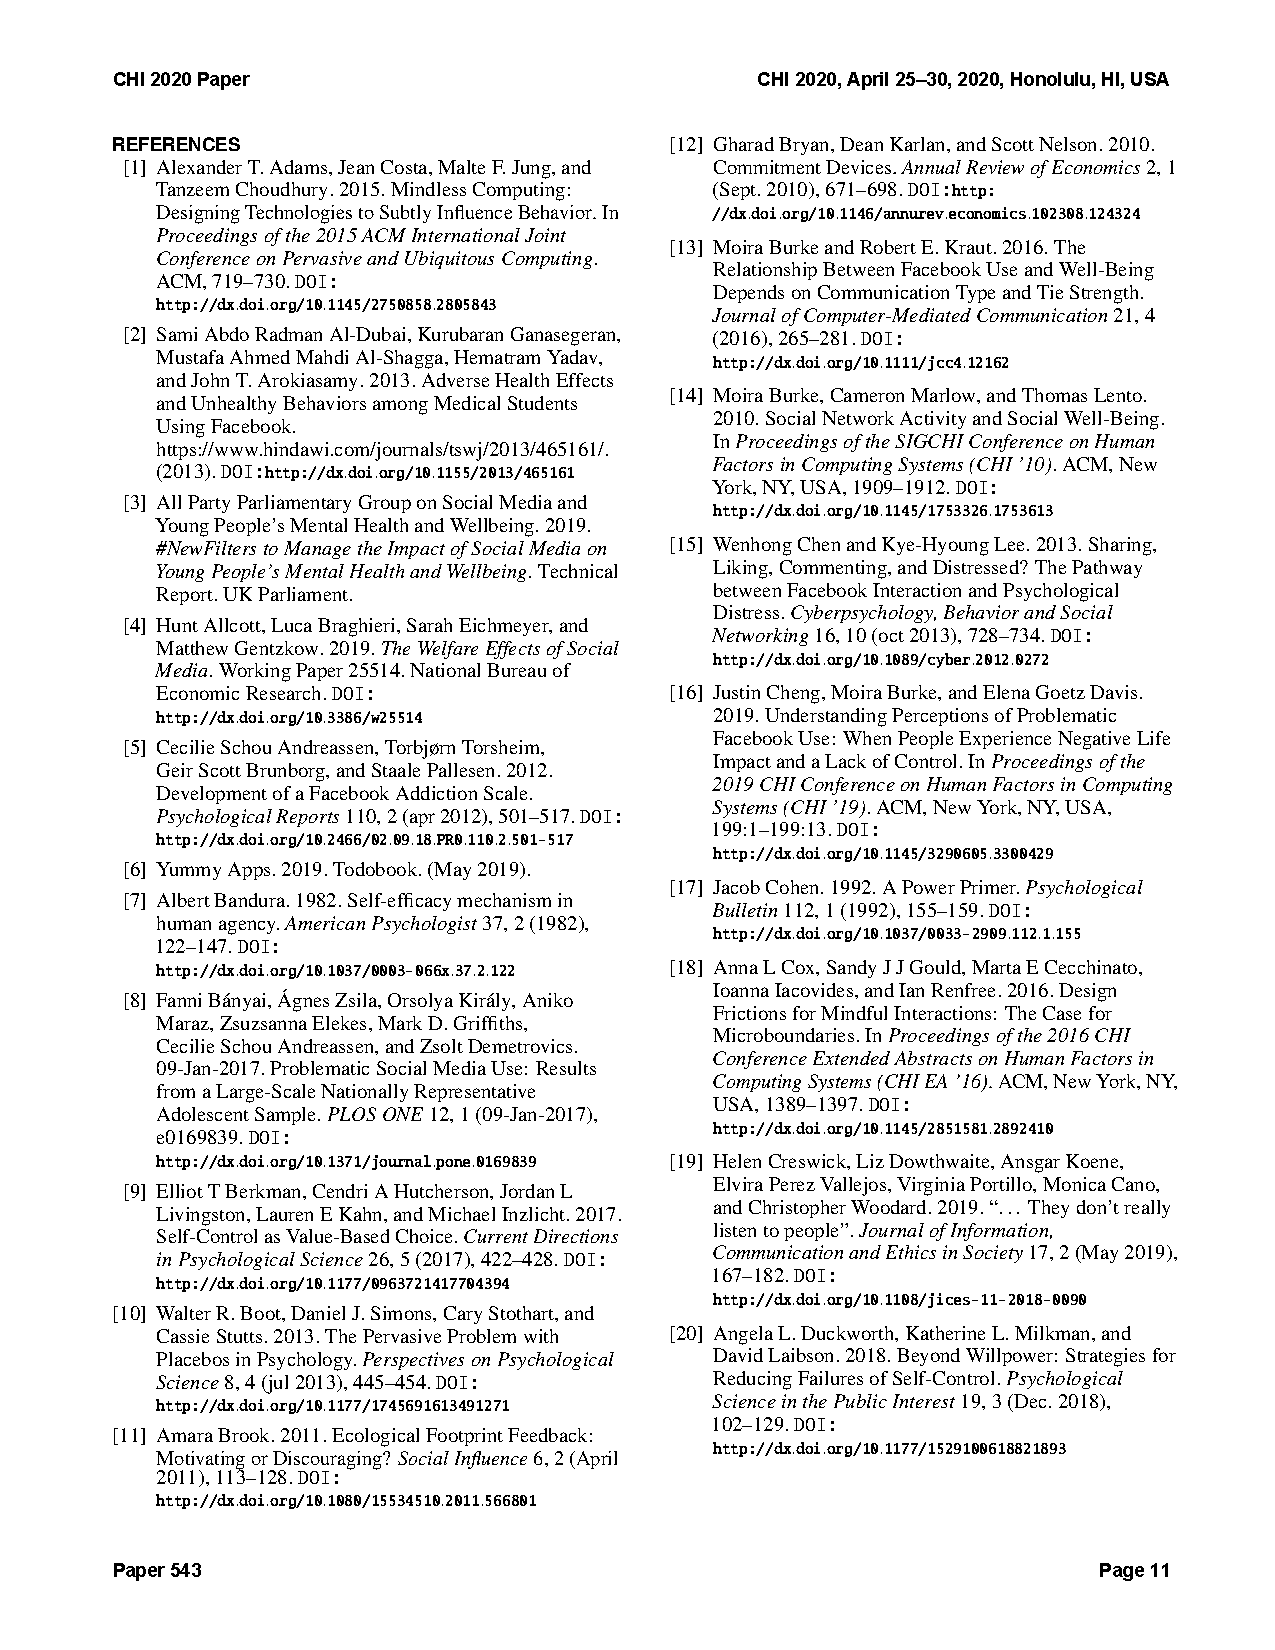
\includegraphics[width=1.2\linewidth]{figures/sample-content/pdf_embed_example/split/_000000000000011.pdf}} \end{center}

\hypertarget{embed-rmd}{%
\section{Including another paper in your thesis - R Markdown child document}\label{embed-rmd}}

Sometimes you want to include another paper you are currently writing as a chapter in your thesis.
Above \ref{embed-pdf}, we described the simplest way to do this: include the other paper as a pdf.
However, in some cases you instead want to include the R Markdown source from this paper, and have it compiled within your thesis.
This is a little bit more tricky, because you need to keep careful track of your file paths, but it is possible by \href{https://bookdown.org/yihui/rmarkdown-cookbook/child-document.html}{including the paper as a child document}.
There are four main steps:

\begin{enumerate}
\def\labelenumi{\arabic{enumi}.}
\tightlist
\item
  Include the paper as a child document
\item
  Make file paths compatible with knitting the article on its own, as well as when it's include in your thesis
\item
  Make header levels correct
\item
  Make figure widths correct
\end{enumerate}

\hypertarget{an-example-paper-in-another-folder}{%
\subsection{An example paper in another folder}\label{an-example-paper-in-another-folder}}

Take this simple example (files for this are in \href{https://github.com/ulyngs/oxforddown-external-article}{this GitHub repository}):

\begin{Shaded}
\begin{Highlighting}[]
\NormalTok{|{-}{-}paper\_to\_include}
\NormalTok{|  |{-}{-}my\_paper.Rmd}
\NormalTok{|  |{-}{-}data}
\NormalTok{|  |  |{-}{-}cat\_salt.csv}
\NormalTok{|  |{-}{-}figures}
\NormalTok{|  |  |{-}{-}cat.jpg}
\NormalTok{|}
\NormalTok{|{-}{-}thesis}
\end{Highlighting}
\end{Shaded}

As the chart suggests, you have another folder, \textbf{paper\_to\_include/} living in the same containing folder as your thesis folder.
In the \textbf{paper\_to\_include} folder, the file \textbf{my\_paper.Rmd} is where you write the paper.
In \textbf{my\_paper.Rmd}, you read in a CSV file found in the subfolder \textbf{data/cats.csv}, and also an image from the subfolder \textbf{figures/cat.jpg}.

\hypertarget{step-1-include-paper-as-a-child-document}{%
\subsection{Step 1: Include paper as a child document}\label{step-1-include-paper-as-a-child-document}}

In your thesis folder, create an Rmd file for the chapter where you want to include another paper.
Add one or more code chunks that include R Markdown files from that paper as child documents:

\begin{Shaded}
\begin{Highlighting}[]
\FunctionTok{\# Including an external chapter }

\InformationTok{\textasciigrave{}\textasciigrave{}\textasciigrave{}\{r child = "../paper\_to\_include/my\_paper.Rmd"\}}
\InformationTok{\textasciigrave{}\textasciigrave{}\textasciigrave{}}
\end{Highlighting}
\end{Shaded}

\hypertarget{step-2-make-file-paths-compatible}{%
\subsection{Step 2: Make file paths compatible}\label{step-2-make-file-paths-compatible}}

Use \href{https://rmarkdown.rstudio.com/lesson-6.html}{parameters} to adjust the file path of images based on values you set in the YAML header of an R Markdown file.
In \textbf{my\_paper.Rmd}, create a parameter called \texttt{other\_path} and set it to an empty string:

\begin{Shaded}
\begin{Highlighting}[]
\PreprocessorTok{{-}{-}{-}}
\FunctionTok{title}\KeywordTok{:}\AttributeTok{ }\StringTok{"A fabulous article in a different folder"}
\FunctionTok{params}\KeywordTok{:}
\AttributeTok{  }\FunctionTok{other\_path}\KeywordTok{:}\AttributeTok{ }\StringTok{""}
\PreprocessorTok{{-}{-}{-}}
\end{Highlighting}
\end{Shaded}

In \textbf{my\_paper.Rmd}, put this at the start of the filepath when you read in data or include images:

\begin{Shaded}
\begin{Highlighting}[]
\FunctionTok{library}\NormalTok{(tidyverse)}
\FunctionTok{library}\NormalTok{(knitr)}

\NormalTok{cat\_data }\OtherTok{\textless{}{-}} \FunctionTok{read\_csv}\NormalTok{(}\FunctionTok{str\_c}\NormalTok{(params}\SpecialCharTok{$}\NormalTok{other\_path, }\StringTok{"data/cats.csv"}\NormalTok{))}
\FunctionTok{include\_graphics}\NormalTok{(}\FunctionTok{str\_c}\NormalTok{(params}\SpecialCharTok{$}\NormalTok{other\_path, }\StringTok{"figures/cat.jpg"}\NormalTok{))}
\end{Highlighting}
\end{Shaded}

Finally, in your thesis folder's \textbf{index.Rmd} file, also create the parameter \texttt{other\_path}.
But here, set it to where the \textbf{paper\_to\_include/} folder is relative to your thesis folder:

\begin{Shaded}
\begin{Highlighting}[]
\FunctionTok{params}\KeywordTok{:}
\AttributeTok{  }\FunctionTok{other\_path}\KeywordTok{:}\AttributeTok{ }\StringTok{"../paper\_to\_include/"}
\end{Highlighting}
\end{Shaded}

\hypertarget{note-on-html-output}{%
\subsubsection{Note on HTML output}\label{note-on-html-output}}

Note that if you want to host an HTML version on your thesis online, you will need to include graphics in the content that you host online - the internet obviously won't be able to see filepaths that are just referring to stuff in another folder on your computer!

\hypertarget{step-3-make-sure-header-levels-are-correct}{%
\subsection{Step 3: Make sure header levels are correct}\label{step-3-make-sure-header-levels-are-correct}}

Unless the paper you want to include is also written as a book, your header levels are probably going to be off.
That is, the level 1 headers (\# Some header) you use for main sections in the other paper turns into chaper titles when included in your thesis.

To avoid this, first \emph{increment all heading levels by one in \textbf{paper\_to\_include/my\_paper.Rmd}} (\# Some header -\textgreater{} \#\# Some header).
Then in \textbf{paper\_to\_include/} create a \href{https://bookdown.org/yihui/rmarkdown-cookbook/lua-filters.html\#lua-filters}{lua filter} that decrements header levels by one: Create a text file, save it as \textbf{reduce\_header\_level.lua}, and give it the content below.

\begin{Shaded}
\begin{Highlighting}[]
\KeywordTok{function}\NormalTok{ Header}\OperatorTok{(}\NormalTok{el}\OperatorTok{)}
  \ControlFlowTok{if} \OperatorTok{(}\NormalTok{el}\OperatorTok{.}\NormalTok{level }\OperatorTok{\textless{}=} \DecValTok{1}\OperatorTok{)} \ControlFlowTok{then}
    \FunctionTok{error}\OperatorTok{(}\StringTok{"I don\textquotesingle{}t know how to decrease the level of h1"}\OperatorTok{)}
  \ControlFlowTok{end}
\NormalTok{  el}\OperatorTok{.}\NormalTok{level }\OperatorTok{=}\NormalTok{ el}\OperatorTok{.}\NormalTok{level }\OperatorTok{{-}} \DecValTok{1}
  \ControlFlowTok{return}\NormalTok{ el}
\KeywordTok{end}
\end{Highlighting}
\end{Shaded}

In the YAML header of \textbf{paper\_to\_include/my\_paper.Rmd}, use this filter:

\begin{Shaded}
\begin{Highlighting}[]
\PreprocessorTok{{-}{-}{-}}
\FunctionTok{title}\KeywordTok{:}\AttributeTok{ }\StringTok{"A fabulous article in a different folder"}
\FunctionTok{params}\KeywordTok{:}
\AttributeTok{  }\FunctionTok{other\_path}\KeywordTok{:}\AttributeTok{ }\StringTok{""}
\FunctionTok{output}\KeywordTok{:}
\AttributeTok{  }\FunctionTok{pdf\_document}\KeywordTok{:}\AttributeTok{ }
\AttributeTok{    }\FunctionTok{pandoc\_args}\KeywordTok{:}\AttributeTok{ }\KeywordTok{[}\StringTok{"{-}{-}lua{-}filter=reduce\_header\_level.lua"}\KeywordTok{]}
\PreprocessorTok{{-}{-}{-}}
\end{Highlighting}
\end{Shaded}

Now, your header levels will be correct both when you knit the paper on its own and when its included in your thesis.

NOTE: There might be no need to use a lua filter to shift heading - it seems you could simply use \texttt{pandoc\_args:\ {[}"-\/-shift-heading-level-by=-1"{]}} (see \url{https://pandoc.org/MANUAL.html\#reader-options})

\hypertarget{step-4.-make-sure-figure-widths-are-correct}{%
\subsection{Step 4. Make sure figure widths are correct}\label{step-4.-make-sure-figure-widths-are-correct}}

It might be that your figure widths when knitting your paper on its own, and when including it in your thesis, need to be different.
You can again use parameters to set figure widths.

Imagine you want figure width to be 80\% of the page width when knitting your paper on its own, but 100\% in your thesis.
In \textbf{paper\_to\_include/my\_paper.Rmd}, first add a parameter we could call \texttt{out\_width} and set it to the string ``80\%'':

\begin{Shaded}
\begin{Highlighting}[]
\PreprocessorTok{{-}{-}{-}}
\FunctionTok{title}\KeywordTok{:}\AttributeTok{ }\StringTok{"A fabulous article in a different folder"}
\FunctionTok{params}\KeywordTok{:}
\AttributeTok{  }\FunctionTok{other\_path}\KeywordTok{:}\AttributeTok{ }\StringTok{""}
\AttributeTok{  }\FunctionTok{out\_width}\KeywordTok{:}\AttributeTok{ }\StringTok{"80\%"}
\FunctionTok{output}\KeywordTok{:}
\AttributeTok{  }\FunctionTok{pdf\_document}\KeywordTok{:}\AttributeTok{ }
\AttributeTok{    }\FunctionTok{pandoc\_args}\KeywordTok{:}\AttributeTok{ }\KeywordTok{[}\StringTok{"{-}{-}lua{-}filter=reduce\_header\_level.lua"}\KeywordTok{]}
\PreprocessorTok{{-}{-}{-}}
\end{Highlighting}
\end{Shaded}

Then, make sure use that parameter to set the output width when you include figures in \textbf{paper\_to\_include/my\_paper.Rmd}:

\begin{Shaded}
\begin{Highlighting}[]
\InformationTok{\textasciigrave{}\textasciigrave{}\textasciigrave{}\{r, out.width=params$out\_width, fig.cap="A very funny cat"\}}
\InformationTok{include\_graphics(str\_c(params$other\_path, "figures/cat.jpg"))}
\InformationTok{\textasciigrave{}\textasciigrave{}\textasciigrave{}}
\end{Highlighting}
\end{Shaded}

Finally, create the parameter \texttt{out\_width} in your thesis' \textbf{index.Rmd} file:

\begin{Shaded}
\begin{Highlighting}[]
\FunctionTok{params}\KeywordTok{:}
\AttributeTok{  }\FunctionTok{other\_path}\KeywordTok{:}\AttributeTok{ }\StringTok{"../paper\_to\_include/"}
\AttributeTok{  }\FunctionTok{out\_width}\KeywordTok{:}\AttributeTok{ }\StringTok{"80\%"}
\end{Highlighting}
\end{Shaded}

Now, the output width of your figure will be 80\% when knitting your paper on its own, and 100\% when knitting it as child document of your thesis.

\hypertarget{customising-citations}{%
\section{Customizing citations and referencing}\label{customising-citations}}

\hypertarget{using-a-.csl-file-with-pandoc}{%
\subsection{Using a .csl file with pandoc}\label{using-a-.csl-file-with-pandoc}}

See section \ref{citation-appearance}.

The only drawbacks to letting pandoc handle citations is that (i) it does not support chapter bibliographies, (ii) if you're a LaTeX veteran, you might be more comfortable with \texttt{biblatex} or \texttt{natbib}.

\hypertarget{biblatex-custom}{%
\subsection{\texorpdfstring{Using \texttt{biblatex}}{Using biblatex}}\label{biblatex-custom}}

To use \href{https://www.overleaf.com/learn/latex/Bibliography_management_with_biblatex}{biblatex} to handle citations, first uncomment this in \textbf{index.Rmd}, YAML header:

\begin{Shaded}
\begin{Highlighting}[]
\AnnotationTok{use{-}biblatex:}\CommentTok{ true}
\AnnotationTok{bib{-}latex{-}options:}\CommentTok{ "style=authoryear, sorting=nyt, backend=biber, maxcitenames=2, useprefix, doi=true, isbn=false, uniquename=false"}
\end{Highlighting}
\end{Shaded}

Then tell R Markdown to use \texttt{biblatex} when inserting citations, by setting \texttt{citation\_package:\ biblatex}:

\begin{Shaded}
\begin{Highlighting}[]
\AnnotationTok{output:}
\NormalTok{  bookdown::pdf\_book:}
\NormalTok{    citation\_package: biblatex}
\end{Highlighting}
\end{Shaded}

To customise the appearance of citations, change \texttt{bib-latex-options}. For example, to get \textbf{numerical citations}, with references in order of their appearance in the text, set it to

\begin{Shaded}
\begin{Highlighting}[]
\AnnotationTok{bib{-}latex{-}options:}\CommentTok{ "style=numeric{-}comp, sorting=none, backend=biber, maxcitenames=2, useprefix, doi=true, isbn=false, uniquename=false"}
\end{Highlighting}
\end{Shaded}

\hypertarget{adding-chapter-bibliographies}{%
\subsubsection{Adding chapter bibliographies}\label{adding-chapter-bibliographies}}

If you would like chapter bibliographies, first add ``refsection=chapter'' to the biblatex options, for example like this:

\begin{Shaded}
\begin{Highlighting}[]
\AnnotationTok{bib{-}latex{-}options:}\CommentTok{ "refsection=chapter, style=authoryear, sorting=nyt, backend=biber, maxcitenames=2, useprefix, doi=true, isbn=false, uniquename=false"}
\end{Highlighting}
\end{Shaded}

Second, set the parameter \texttt{insertHeadingInPDF:\ false} in \textbf{index.Rmd}, to suppress the inclusion of a `References' heading at the end of the thesis.

\begin{Shaded}
\begin{Highlighting}[]
\AnnotationTok{params:}
\NormalTok{  insertHeadingInPDF: false}
\end{Highlighting}
\end{Shaded}

Finally insert this line at the end of each chapter, to print the bibliographies there:

\begin{Shaded}
\begin{Highlighting}[]
\FunctionTok{\textbackslash{}printbibliography}\NormalTok{[segment=}\FunctionTok{\textbackslash{}therefsection}\NormalTok{,heading=subbibliography]}
\end{Highlighting}
\end{Shaded}

\hypertarget{natbib-custom}{%
\subsection{\texorpdfstring{Using \texttt{natbib}}{Using natbib}}\label{natbib-custom}}

To use \href{https://www.overleaf.com/learn/latex/Bibliography_management_with_natbib}{natbib} to handle citations, first uncomment this in \textbf{index.Rmd}, YAML header:

\begin{Shaded}
\begin{Highlighting}[]
\AnnotationTok{use{-}natbib:}\CommentTok{ true}
\AnnotationTok{natbib{-}citation{-}style:}\CommentTok{ authoryear \#for science, you might want numbers,square}
\AnnotationTok{natbib{-}bibliography{-}style:}\CommentTok{ templates/ACM{-}Reference{-}Format.bst \#e.g. "plainnat", unsrtnat, or path to a .bst file}
\end{Highlighting}
\end{Shaded}

Then tell R Markdown to use \texttt{natbib} when inserting citations, by setting \texttt{citation\_package:\ natbib}:

\begin{Shaded}
\begin{Highlighting}[]
\AnnotationTok{output:}
\NormalTok{  bookdown::pdf\_book:}
\NormalTok{    citation\_package: natbib}
\end{Highlighting}
\end{Shaded}

To customise the appearance of citations, change what \textbf{.bst} file you point to in \texttt{natbib-bibliography-style}.

\hypertarget{customizing-the-page-headers-and-footers-pdf}{%
\section{Customizing the page headers and footers (PDF)}\label{customizing-the-page-headers-and-footers-pdf}}

This can now be done directly in \textbf{index.Rmd}'s YAML header.
If you are a LaTeX expert and need further customisation that what's currently provided, you can tweak the relevant sections of \textbf{templates/template.tex} - the relevant code is beneath the line that begins \texttt{\textbackslash{}usepackage\{fancyhdr\}}.

\hypertarget{diving-in-to-the-oxthesis-latex-template-pdf}{%
\section{Diving in to the OxThesis LaTeX template (PDF)}\label{diving-in-to-the-oxthesis-latex-template-pdf}}

For LaTeX minded people, you can read through \textbf{templates/template.tex} to see which additional customisation options are available as well as \textbf{templates/ociamthesis.cls} which supplies the base class.
For example, \textbf{template.tex} provides an option for master's degree submissions, which changes identifying information to candidate number and includes a word count.
At the time of writing, you must set this directly in \textbf{template.tex} rather than from the YAML header in \textbf{index.Rmd}.

\hypertarget{customising-to-a-different-university}{%
\section{Customising to a different university}\label{customising-to-a-different-university}}

\hypertarget{the-minimal-route}{%
\subsection{The minimal route}\label{the-minimal-route}}

If the front matter in the OxThesis LaTeX template is suitable to your university, customising \texttt{oxforddown} to your needs could be as simple as putting the name of your institution and the path to your university's logo in \textbf{index.Rmd}:

\begin{Shaded}
\begin{Highlighting}[]
\FunctionTok{university}\KeywordTok{:}\AttributeTok{ University of You}
\FunctionTok{university{-}logo}\KeywordTok{:}\AttributeTok{ figures/your{-}logo{-}here.pdf}
\end{Highlighting}
\end{Shaded}

\hypertarget{replacing-the-entire-title-page-with-your-required-content}{%
\subsection{Replacing the entire title page with your required content}\label{replacing-the-entire-title-page-with-your-required-content}}

If you have a \textbf{.tex} file with some required front matter from your university that you want to replace the OxThesis template's title page altogether, you can provide a filepath to this file in \textbf{index.Rmd}.
\texttt{oxforddown}'s sample content includes and example of this --- if you use the YAML below, your front matter will look like this:

\begin{Shaded}
\begin{Highlighting}[]
\FunctionTok{alternative{-}title{-}page}\KeywordTok{:}\AttributeTok{ front{-}and{-}back{-}matter/alt{-}title{-}page{-}example.tex}
\end{Highlighting}
\end{Shaded}

\noindent
\fbox{
\includegraphics[width=0.32\linewidth]{figures/sample-content/alt_frontmatter_example/split/_000001.pdf}} \fbox{
\includegraphics[width=0.32\linewidth]{figures/sample-content/alt_frontmatter_example/split/_000002.pdf}} \fbox{
\includegraphics[width=0.32\linewidth]{figures/sample-content/alt_frontmatter_example/split/_000003.pdf}} \fbox{
\includegraphics[width=0.32\linewidth]{figures/sample-content/alt_frontmatter_example/split/_000004.pdf}} \fbox{
\includegraphics[width=0.32\linewidth]{figures/sample-content/alt_frontmatter_example/split/_000005.pdf}} \fbox{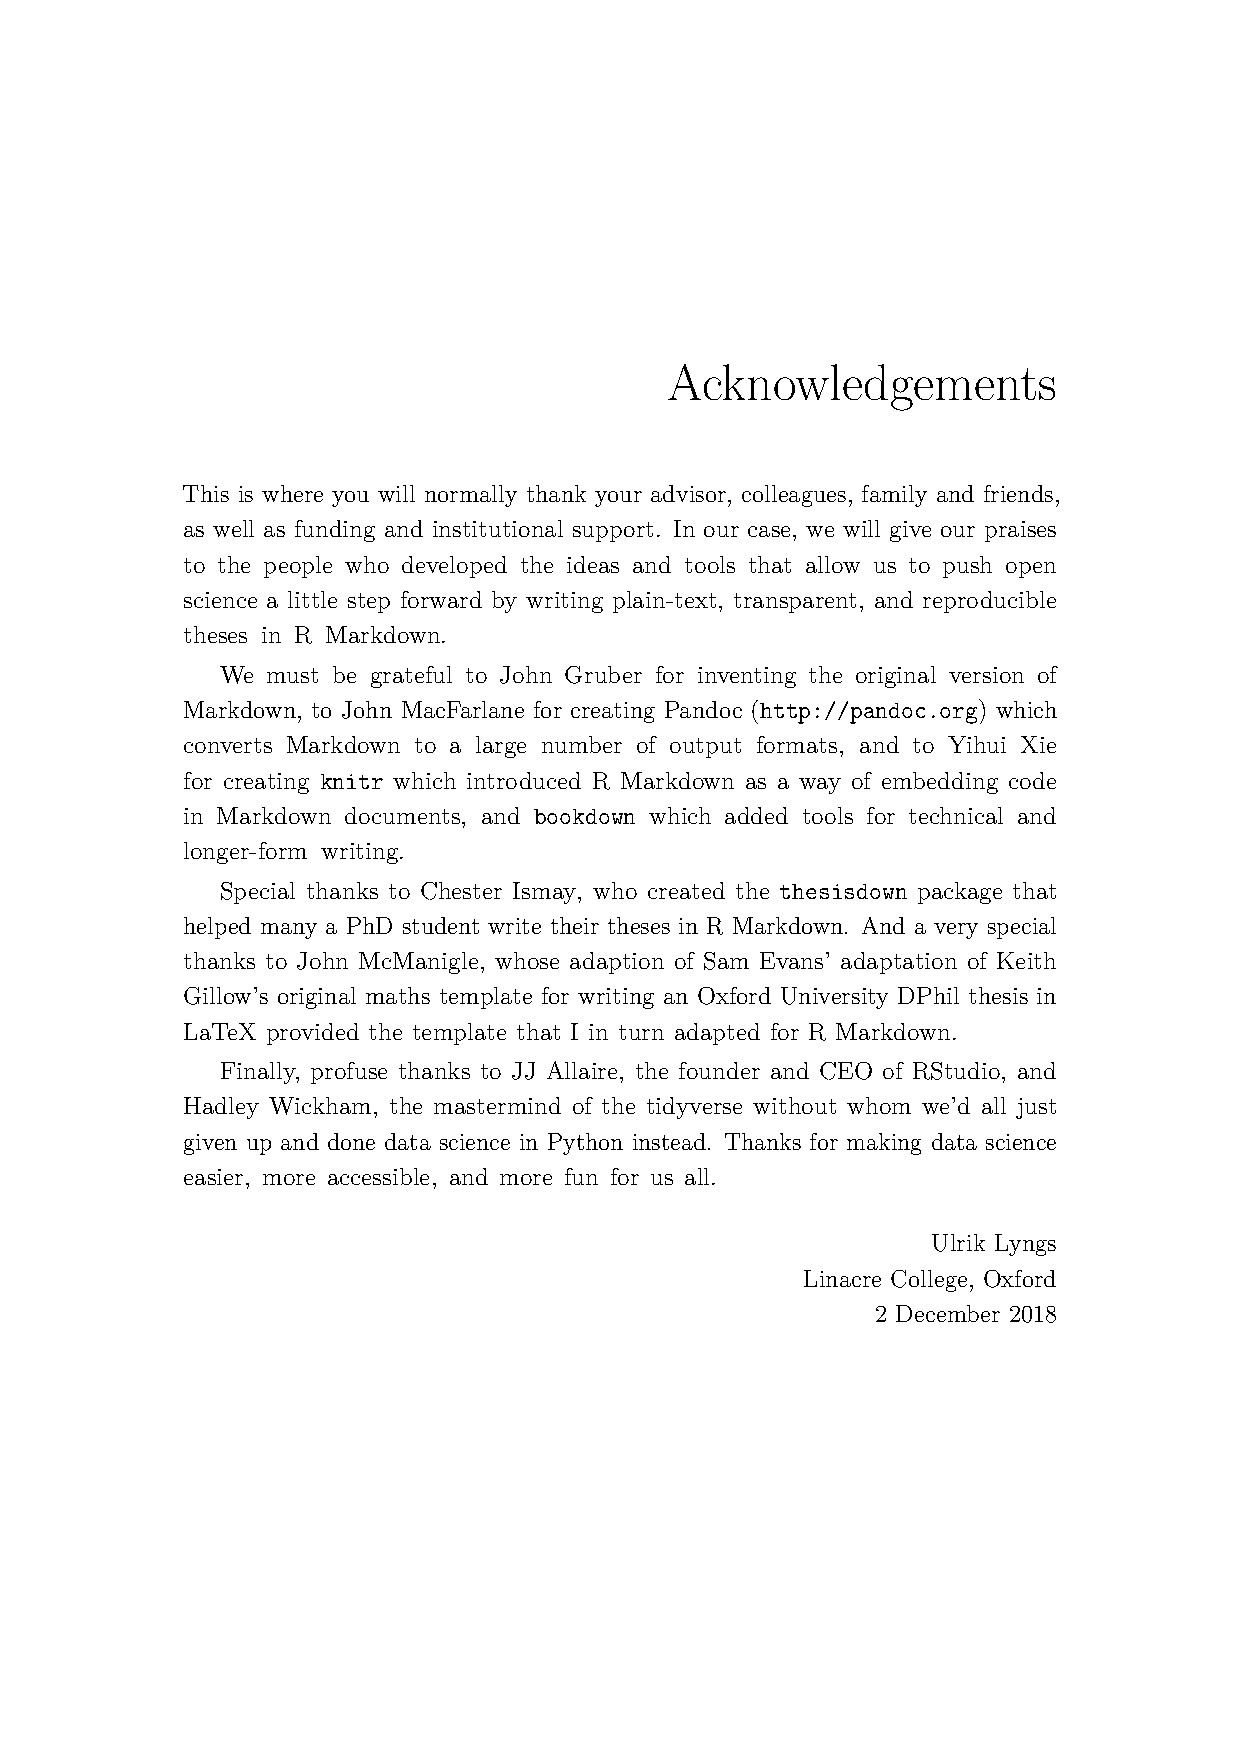
\includegraphics[width=0.32\linewidth]{figures/sample-content/alt_frontmatter_example/split/_000006.pdf}}



\hypertarget{conclusion}{%
\chapter*{Conclusion}\label{conclusion}}
\addcontentsline{toc}{chapter}{Conclusion}

If we don't want Conclusion to have a chapter number next to it, we can add the \texttt{\{-\}} attribute.

\hypertarget{more-info}{%
\section*{More info}\label{more-info}}
\addcontentsline{toc}{section}{More info}

And here's some other random info:
the first paragraph after a chapter title or section head \emph{shouldn't be} indented, because indents are to tell the reader that you're starting a new paragraph.
Since that's obvious after a chapter or section title, proper typesetting doesn't add an indent there.

This paragraph, by contrast, \emph{will} be indented as it should because it is not the first one after the `More info' heading.
All hail LaTeX. (If you're reading the HTML version, you won't see any indentation - have a look at the PDF version to understand what in the earth this section is babbling on about).

\startappendices

\hypertarget{the-first-appendix}{%
\chapter{The First Appendix}\label{the-first-appendix}}

This first appendix includes an R chunk that was hidden in the document (using \texttt{echo\ =\ FALSE}) to help with readibility:

\textbf{In 02-rmd-basics-code.Rmd}

\begin{Shaded}
\begin{Highlighting}[]
\FunctionTok{library}\NormalTok{(tidyverse)}
\NormalTok{knitr}\SpecialCharTok{::}\FunctionTok{include\_graphics}\NormalTok{(}\StringTok{"figures/sample{-}content/chunk{-}parts.png"}\NormalTok{)}
\end{Highlighting}
\end{Shaded}

\textbf{And here's another one from the same chapter, i.e.~Chapter \ref{code}:}

\begin{Shaded}
\begin{Highlighting}[]
\NormalTok{knitr}\SpecialCharTok{::}\FunctionTok{include\_graphics}\NormalTok{(}\StringTok{"figures/sample{-}content/beltcrest.png"}\NormalTok{)}
\end{Highlighting}
\end{Shaded}

\hypertarget{the-second-appendix-for-fun}{%
\chapter{The Second Appendix, for Fun}\label{the-second-appendix-for-fun}}

\hypertarget{references}{%
\chapter*{References}\label{references}}
\addcontentsline{toc}{chapter}{References}

\markboth{References}{}

\hypertarget{refs}{}
\begin{CSLReferences}{1}{0}
\leavevmode\vadjust pre{\hypertarget{ref-Darwin1859}{}}%
Darwin, C. (1859). \emph{{On the Origin of Species by Means of Natural Selection or the Preservation of Favoured Races in the Struggle for Life}}. John Murray.

\leavevmode\vadjust pre{\hypertarget{ref-von_goethe_wilhelm_1829}{}}%
Goethe, J. W. von. (1829). \emph{Wilhelm {Meisters} {Wanderjahre} oder die {Entsagenden}}. Cotta.

\leavevmode\vadjust pre{\hypertarget{ref-Lottridge2012}{}}%
Lottridge, D., Marschner, E., Wang, E., Romanovsky, M., \& Nass, C. (2012). {Browser design impacts multitasking}. \emph{Proceedings of the Human Factors and Ergonomics Society 56th Annual Meeting}. \url{https://doi.org/10.1177/1071181312561289}

\leavevmode\vadjust pre{\hypertarget{ref-Mill1965}{}}%
Mill, J. S. (1965 {[}1843{]}). \emph{A system of logic, ratiocinative and inductive: Being a connected view of the principles of evidence and the methods of scientific investigation}. Longmans.

\leavevmode\vadjust pre{\hypertarget{ref-Shea2014}{}}%
Shea, N., Boldt, A., Bang, D., Yeung, N., Heyes, C., \& Frith, C. D. (2014). {Supra-personal cognitive control and metacognition}. \emph{Trends in Cognitive Sciences}, \emph{18}(4), 186--193. \url{https://doi.org/10.1016/j.tics.2014.01.006}

\leavevmode\vadjust pre{\hypertarget{ref-Wu2016}{}}%
Wu, T. (2016). \emph{{The Attention Merchants: The Epic Scramble to Get Inside Our Heads}}. Knopf Publishing Group.

\end{CSLReferences}

%%%%% REFERENCES


\end{document}
